% Options for packages loaded elsewhere
\PassOptionsToPackage{unicode}{hyperref}
\PassOptionsToPackage{hyphens}{url}
%
\documentclass[
]{article}
\usepackage{amsmath,amssymb}
\usepackage{iftex}
\ifPDFTeX
  \usepackage[T1]{fontenc}
  \usepackage[utf8]{inputenc}
  \usepackage{textcomp} % provide euro and other symbols
\else % if luatex or xetex
  \usepackage{unicode-math} % this also loads fontspec
  \defaultfontfeatures{Scale=MatchLowercase}
  \defaultfontfeatures[\rmfamily]{Ligatures=TeX,Scale=1}
\fi
\usepackage{lmodern}
\ifPDFTeX\else
  % xetex/luatex font selection
\fi
% Use upquote if available, for straight quotes in verbatim environments
\IfFileExists{upquote.sty}{\usepackage{upquote}}{}
\IfFileExists{microtype.sty}{% use microtype if available
  \usepackage[]{microtype}
  \UseMicrotypeSet[protrusion]{basicmath} % disable protrusion for tt fonts
}{}
\makeatletter
\@ifundefined{KOMAClassName}{% if non-KOMA class
  \IfFileExists{parskip.sty}{%
    \usepackage{parskip}
  }{% else
    \setlength{\parindent}{0pt}
    \setlength{\parskip}{6pt plus 2pt minus 1pt}}
}{% if KOMA class
  \KOMAoptions{parskip=half}}
\makeatother
\usepackage{xcolor}
\usepackage[margin=1in]{geometry}
\usepackage{color}
\usepackage{fancyvrb}
\newcommand{\VerbBar}{|}
\newcommand{\VERB}{\Verb[commandchars=\\\{\}]}
\DefineVerbatimEnvironment{Highlighting}{Verbatim}{commandchars=\\\{\}}
% Add ',fontsize=\small' for more characters per line
\usepackage{framed}
\definecolor{shadecolor}{RGB}{248,248,248}
\newenvironment{Shaded}{\begin{snugshade}}{\end{snugshade}}
\newcommand{\AlertTok}[1]{\textcolor[rgb]{0.94,0.16,0.16}{#1}}
\newcommand{\AnnotationTok}[1]{\textcolor[rgb]{0.56,0.35,0.01}{\textbf{\textit{#1}}}}
\newcommand{\AttributeTok}[1]{\textcolor[rgb]{0.13,0.29,0.53}{#1}}
\newcommand{\BaseNTok}[1]{\textcolor[rgb]{0.00,0.00,0.81}{#1}}
\newcommand{\BuiltInTok}[1]{#1}
\newcommand{\CharTok}[1]{\textcolor[rgb]{0.31,0.60,0.02}{#1}}
\newcommand{\CommentTok}[1]{\textcolor[rgb]{0.56,0.35,0.01}{\textit{#1}}}
\newcommand{\CommentVarTok}[1]{\textcolor[rgb]{0.56,0.35,0.01}{\textbf{\textit{#1}}}}
\newcommand{\ConstantTok}[1]{\textcolor[rgb]{0.56,0.35,0.01}{#1}}
\newcommand{\ControlFlowTok}[1]{\textcolor[rgb]{0.13,0.29,0.53}{\textbf{#1}}}
\newcommand{\DataTypeTok}[1]{\textcolor[rgb]{0.13,0.29,0.53}{#1}}
\newcommand{\DecValTok}[1]{\textcolor[rgb]{0.00,0.00,0.81}{#1}}
\newcommand{\DocumentationTok}[1]{\textcolor[rgb]{0.56,0.35,0.01}{\textbf{\textit{#1}}}}
\newcommand{\ErrorTok}[1]{\textcolor[rgb]{0.64,0.00,0.00}{\textbf{#1}}}
\newcommand{\ExtensionTok}[1]{#1}
\newcommand{\FloatTok}[1]{\textcolor[rgb]{0.00,0.00,0.81}{#1}}
\newcommand{\FunctionTok}[1]{\textcolor[rgb]{0.13,0.29,0.53}{\textbf{#1}}}
\newcommand{\ImportTok}[1]{#1}
\newcommand{\InformationTok}[1]{\textcolor[rgb]{0.56,0.35,0.01}{\textbf{\textit{#1}}}}
\newcommand{\KeywordTok}[1]{\textcolor[rgb]{0.13,0.29,0.53}{\textbf{#1}}}
\newcommand{\NormalTok}[1]{#1}
\newcommand{\OperatorTok}[1]{\textcolor[rgb]{0.81,0.36,0.00}{\textbf{#1}}}
\newcommand{\OtherTok}[1]{\textcolor[rgb]{0.56,0.35,0.01}{#1}}
\newcommand{\PreprocessorTok}[1]{\textcolor[rgb]{0.56,0.35,0.01}{\textit{#1}}}
\newcommand{\RegionMarkerTok}[1]{#1}
\newcommand{\SpecialCharTok}[1]{\textcolor[rgb]{0.81,0.36,0.00}{\textbf{#1}}}
\newcommand{\SpecialStringTok}[1]{\textcolor[rgb]{0.31,0.60,0.02}{#1}}
\newcommand{\StringTok}[1]{\textcolor[rgb]{0.31,0.60,0.02}{#1}}
\newcommand{\VariableTok}[1]{\textcolor[rgb]{0.00,0.00,0.00}{#1}}
\newcommand{\VerbatimStringTok}[1]{\textcolor[rgb]{0.31,0.60,0.02}{#1}}
\newcommand{\WarningTok}[1]{\textcolor[rgb]{0.56,0.35,0.01}{\textbf{\textit{#1}}}}
\usepackage{longtable,booktabs,array}
\usepackage{calc} % for calculating minipage widths
% Correct order of tables after \paragraph or \subparagraph
\usepackage{etoolbox}
\makeatletter
\patchcmd\longtable{\par}{\if@noskipsec\mbox{}\fi\par}{}{}
\makeatother
% Allow footnotes in longtable head/foot
\IfFileExists{footnotehyper.sty}{\usepackage{footnotehyper}}{\usepackage{footnote}}
\makesavenoteenv{longtable}
\usepackage{graphicx}
\makeatletter
\def\maxwidth{\ifdim\Gin@nat@width>\linewidth\linewidth\else\Gin@nat@width\fi}
\def\maxheight{\ifdim\Gin@nat@height>\textheight\textheight\else\Gin@nat@height\fi}
\makeatother
% Scale images if necessary, so that they will not overflow the page
% margins by default, and it is still possible to overwrite the defaults
% using explicit options in \includegraphics[width, height, ...]{}
\setkeys{Gin}{width=\maxwidth,height=\maxheight,keepaspectratio}
% Set default figure placement to htbp
\makeatletter
\def\fps@figure{htbp}
\makeatother
\usepackage{svg}
\setlength{\emergencystretch}{3em} % prevent overfull lines
\providecommand{\tightlist}{%
  \setlength{\itemsep}{0pt}\setlength{\parskip}{0pt}}
\setcounter{secnumdepth}{-\maxdimen} % remove section numbering
\ifLuaTeX
  \usepackage{selnolig}  % disable illegal ligatures
\fi
\IfFileExists{bookmark.sty}{\usepackage{bookmark}}{\usepackage{hyperref}}
\IfFileExists{xurl.sty}{\usepackage{xurl}}{} % add URL line breaks if available
\urlstyle{same}
\hypersetup{
  pdftitle={Barcelona Airbnb Insights},
  pdfauthor={Daniel Herrera \& Rodrigo González},
  hidelinks,
  pdfcreator={LaTeX via pandoc}}

\title{Barcelona Airbnb Insights}
\author{Daniel Herrera \& Rodrigo González}
\date{2024-02-10}

\begin{document}
\maketitle

\hypertarget{presentation-of-the-case}{%
\subsection{1. Presentation of the
case}\label{presentation-of-the-case}}

\includesvg[width=0.25\textwidth,height=\textheight]{Assets/Airbnb_Logo_Bélo.svg}

\hypertarget{airbnb}{%
\subsubsection{1.1. Airbnb}\label{airbnb}}

Airbnb, founded in 2008, has grown from a simple idea of renting out air
mattresses in a San Francisco apartment to a global phenomenon in the
hospitality industry. It has significantly altered the way people travel
by offering unique accommodations from local hosts in over 100,000
cities worldwide. Its platform caters to a diverse range of preferences,
from single rooms to entire homes, providing more personalized and often
more cost-effective lodging options than traditional hotels. This
peer-to-peer model has not only democratized travel accommodations but
also enabled millions of hosts to generate additional income. As of
2022, Airbnb had hosted over 800 million guest arrivals, showcasing its
vast growth and popularity among travelers seeking authentic
experiences. This growth trajectory highlights Airbnb's impact on the
travel and tourism sector, prompting a reevaluation of traditional
hospitality models and regulatory frameworks globally.

\begin{center}\rule{0.5\linewidth}{0.5pt}\end{center}

\hypertarget{airbnb-controversies}{%
\subsubsection{1.2. Airbnb controversies}\label{airbnb-controversies}}

Airbnb's rise has sparked controversies, especially around its impact on
local housing markets, community dynamics, and regulatory compliance.
The platform has been criticized for contributing to housing shortages
by converting long-term rental properties into short-term tourist
accommodations, leading to increased rent and property prices. In cities
like Barcelona, this has exacerbated existing tensions between residents
and tourists, contributing to over-tourism and altering neighborhood
characters. Additionally, Airbnb has faced legal challenges regarding
compliance with local housing laws and regulations, with accusations of
facilitating illegal rentals. These issues have prompted cities
worldwide to implement stricter regulations on short-term rentals,
balancing the need for tourism revenue with protecting residents'
interests and preserving housing affordability.

Recently, Airbnb has seen a noticeable increase in rental prices,
attributed to a combination of factors including heightened demand,
limited supply, and the gradual recovery of the travel industry
post-pandemic. This surge reflects a broader trend in the accommodation
sector where prices are climbing as travelers return in large numbers,
seeking unique and safe lodging options. The rise in prices has sparked
discussions on affordability and access, urging both Airbnb and hosts to
balance profitability with providing value to guests.

\begin{center}\rule{0.5\linewidth}{0.5pt}\end{center}

\hypertarget{airbnb-in-barcelona}{%
\subsubsection{1.3. Airbnb in Barcelona}\label{airbnb-in-barcelona}}

Airbnb's controversies in Barcelona have been a focal point of
discussions about the impact of short-term rentals on cities globally.
Barcelona, a prime tourist destination, has faced significant challenges
due to the proliferation of Airbnb listings, leading to tensions between
the platform, the city's residents, and local authorities.

One major controversy revolves around housing affordability and
availability. Critics argue that Airbnb contributes to rising rents and
the displacement of long-term residents in favor of short-term tourists.
The city has seen protests from local groups and activists who claim
that neighborhoods have lost their identity and cohesion due to the
influx of tourists staying in Airbnb properties. These concerns have
been echoed by housing advocacy groups like the Platform for People
Affected by Mortgages (PAH), which has been vocal about the negative
impacts of short-term rentals on the local housing market.

The Barcelona City Council, led by Mayor Ada Colau, has taken a firm
stance against illegal tourist rentals. Since coming to office in 2015,
Colau has introduced strict regulations aimed at curbing the growth of
short-term rental platforms like Airbnb. In 2016, the city imposed a
moratorium on new tourist licenses and fined Airbnb €600,000 for listing
unlicensed properties, highlighting the city's commitment to enforcing
its regulations.

Further actions were taken in subsequent years, including the
introduction of the PEUAT (Special Urban Plan for Tourist Accommodation)
in 2017, which aimed to limit the expansion of tourist accommodations
and ensure a balance between tourism and local residents' needs. Despite
these measures, conflicts persist, with Airbnb arguing that the city's
approach is overly restrictive and harms local hosts who rely on income
from short-term rentals.

\begin{center}\rule{0.5\linewidth}{0.5pt}\end{center}

\hypertarget{data-sources}{%
\subsubsection{1.4. Data sources}\label{data-sources}}

Despite the significance of Airbnb data, the private nature of the
company, being publicly listed, rules out its open publication.
Consequently, an alternative approach is necessary for data collection.
In this report, we opt to depend on robust and reliable projects that
have already proven their significance in regulating this reservation
platform, as well as data sourced directly from the municipality.

We have established two distinct sources of data, the first involves the
\emph{Inside Airbnb} project, while the second is taken from the Open
Data portal of the Barcelona City Council.


\includegraphics[width=0.25\textwidth,height=\textheight]{Assets/InsideAirbnb.png}

\hypertarget{inside-airbnb}{%
\paragraph{1.4.1. Inside Airbnb}\label{inside-airbnb}}

The \href{http://insideairbnb.com/}{Inside Airbnb} project is a
comprehensive, independent online platform that provides data and
analysis on the operations of Airbnb in cities around the world. It was
started by activist and data scientist Murray Cox in 2016 as a response
to the lack of transparency regarding how Airbnb's business model
impacts local housing markets, neighborhoods, and communities. The
project aggregates publicly available information on Airbnb listings and
reviews to present a more detailed picture of the platform's presence in
various cities.

Inside Airbnb has become a crucial resource for researchers,
policymakers, journalists, and community groups concerned about the
rapid growth of short-term rentals and their effect on cities. By
offering detailed data on the number of listings, types of properties,
location, pricing, and host information, the project sheds light on how
Airbnb contributes to issues like housing affordability, gentrification,
and regulatory compliance.

One of the most significant repercussions of the Inside Airbnb project
has been its influence on public policy and regulation. Cities like New
York, San Francisco, and Barcelona have used data from Inside Airbnb to
understand the scale and impact of short-term rentals, leading to the
development and enforcement of more stringent short-term rental
regulations. For instance, New York City has implemented rules requiring
hosts to register with the city, a move aimed at cracking down on
illegal listings---a policy informed by insights gained from Inside
Airbnb's data.

Inside Airbnb's work has not been without criticism, particularly from
Airbnb and hosts who argue that the platform's data might be
misinterpreted or used to unjustifiably restrict short-term rentals.
Nonetheless, the project's impact in highlighting the need for balance
between tourism benefits and community well-being remains undeniable.

In our case we have used the data set of the city of Barcelona through
two files, one being the facelifts and the other being the GEOJson of
the locations. The quality of the data is indisputable and has been
recognized by various actors. Likewise, the update is continuous and we
work with data from less than two months ago, these being from
mid-December.

We thank Inside Airbnb for its collaboration with consumers and the
governments in making this data public, easily reachable and visible.


\includegraphics[width=0.25\textwidth,height=\textheight]{Assets/OpenDataBCN.png}

\hypertarget{open-data-bcn}{%
\paragraph{1.4.2. Open data BCN}\label{open-data-bcn}}

The portal \url{https://opendata-ajuntament.barcelona.cat/} is an
initiative by the Barcelona City Council aimed at promoting
transparency, citizen participation, and innovation through open access
to public data. This digital platform offers a wide array of datasets on
various city aspects such as transportation, environment, demographics,
and economy, enabling developers, researchers, and the general public to
analyze, create, and share applications that enhance the understanding
and management of the city.

In our case we have used the data set of ``Population of Barcelona
aggregated by sex according to the Municipal Register of Inhabitants on
January 1 of each year''. Barcelona City Council offers an easy-to-use
API from which we have only indexed the fields of our interest.

We thank Barcelona City Council for its collaboration with citizens and
general public for publishing this data of general interest.

\url{https://opendata-ajuntament.barcelona.cat/data/en/dataset/pad_mdbas_sexe/resource/d0e4ec78-e274-4300-a3bc-cb85cf79014d}

\begin{center}\rule{0.5\linewidth}{0.5pt}\end{center}


\includegraphics[width=0.25\textwidth,height=\textheight]{Assets/OMIC.png}

\hypertarget{municipal-consumer-information-office-omic}{%
\subsubsection{1.5. Municipal Consumer Information Office
(OMIC)}\label{municipal-consumer-information-office-omic}}

The Municipal Consumer Information Office (OMIC) in Barcelona plays a
crucial role in protecting consumer rights within the city. This
institution provides essential services such as advice, mediation, and
conflict resolution between consumers and businesses. Established to
ensure that consumer rights are respected and promoted, OMIC offers a
valuable resource for citizens facing issues with products or services.

OMIC operates in various areas, including handling complaints and
claims, promoting responsible consumption practices, and educating about
consumer rights. It also offers workshops and informative talks,
contributing to raising awareness and educating consumers about their
rights and how to effectively exercise them.

Additionally, OMIC monitors commercial practices within the city to
ensure compliance with current consumer legislation. This includes
inspecting commercial establishments and implementing corrective actions
in cases of infringement. Its work is essential in maintaining a fair
balance between consumer interests and those of businesses, promoting a
transparent and fair market.

We consider that OMIC is the perfect client for a report that reflects
the impact that Airbnb is having on the city of Barcelona. Likewise, and
after the major controversies over the price increase that Airbnb has
had lately, it is interesting to observe the profile of accommodation
and large license holders that Barcelona City Council has had under its
sights for years.

This study is the first phase and after adequate negotiation a second
could be launched with much more detailed data.

\begin{center}\rule{0.5\linewidth}{0.5pt}\end{center}

\hypertarget{data-exploration}{%
\subsection{2. Data exploration}\label{data-exploration}}

\hypertarget{data-structure}{%
\subsubsection{2.1. Data structure}\label{data-structure}}

\hypertarget{inside-airbnb-1}{%
\paragraph{2.1.1 Inside Airbnb}\label{inside-airbnb-1}}

Each entry collected by Inside Airbnb, corresponding to one geographical
location or city, is structured unanimously in the following manner:

\begin{longtable}[]{@{}
  >{\raggedright\arraybackslash}p{(\columnwidth - 4\tabcolsep) * \real{0.3103}}
  >{\raggedright\arraybackslash}p{(\columnwidth - 4\tabcolsep) * \real{0.3448}}
  >{\raggedright\arraybackslash}p{(\columnwidth - 4\tabcolsep) * \real{0.3448}}@{}}
\toprule\noalign{}
\begin{minipage}[b]{\linewidth}\raggedright
Country/City
\end{minipage} & \begin{minipage}[b]{\linewidth}\raggedright
File Name
\end{minipage} & \begin{minipage}[b]{\linewidth}\raggedright
Description
\end{minipage} \\
\midrule\noalign{}
\endhead
\bottomrule\noalign{}
\endlastfoot
Barcelona & listings.csv.gz & Detailed Listings data \\
Barcelona & calendar.csv.gz & Detailed Calendar Data \\
Barcelona & reviews.csv.gz & Detailed Review Data \\
Barcelona & listings.csv & Summary information and metrics for listings
in (good for visualisations). \\
Barcelona & reviews.csv & Summary Review data and Listing ID (to
facilitate time based analytics and visualisations linked to a
listing). \\
Barcelona & neighbourhoods.csv & Neighbourhood list for geo filter.
Sourced from city or open source GIS files. \\
Barcelona & neighbourhoods.geojson & GeoJSON file of neighbourhoods of
the city. \\
\end{longtable}

Given this recurring structure and the richness of the data, the initial
goal of the project was to compare data from different European cities.
This objective is evident in the code implementation for loading data
into data frames, designed to be replicable and applicable to any city's
data, provided the files are loaded into the working directory and
stored in folders named after the respective cities. This approach was
eventually discarded, as it became clear that focusing on Barcelona as a
study case is already in itself an interesting focus.

The data collected from Barcelona corresponds to the 13 of December,
2023.

The main source of data is the \texttt{listings.csv} file, which
contains a collection of 18,321 listings with 18 variables:

\begin{Shaded}
\begin{Highlighting}[]
\FunctionTok{dim}\NormalTok{(Barcelona)}
\end{Highlighting}
\end{Shaded}

\begin{verbatim}
## [1] 18321    18
\end{verbatim}

\begin{Shaded}
\begin{Highlighting}[]
\FunctionTok{str}\NormalTok{(Barcelona)}
\end{Highlighting}
\end{Shaded}

\begin{verbatim}
## 'data.frame':    18321 obs. of  18 variables:
##  $ id                            : num  17475 18674 198958 23197 32711 ...
##  $ name                          : chr  "Rental unit in 08013 Barcelona · ★4.40 · 1 bedroom · 1 bed · 1 bath" "Rental unit in Barcelona · ★4.33 · 3 bedrooms · 6 beds · 2 baths" "Rental unit in Barcelona · ★4.69 · 4 bedrooms · 6 beds · 2 baths" "Rental unit in Sant Adria de Besos · ★4.77 · 3 bedrooms · 4 beds · 2 baths" ...
##  $ host_id                       : int  65623 71615 971768 90417 135703 440825 73163 1013855 1014050 73163 ...
##  $ host_name                     : chr  "Luca" "Mireia  Maria" "Laura" "Etain (Marnie)" ...
##  $ neighbourhood_group           : chr  "Eixample" "Eixample" "Sant Martí" "Sant Martí" ...
##  $ neighbourhood                 : chr  "la Dreta de l'Eixample" "la Sagrada Família" "Diagonal Mar i el Front Marítim del Poblenou" "el Besòs i el Maresme" ...
##  $ latitude                      : num  41.4 41.4 41.4 41.4 41.4 ...
##  $ longitude                     : num  2.17 2.17 2.21 2.22 2.17 ...
##  $ room_type                     : chr  "Entire home/apt" "Entire home/apt" "Entire home/apt" "Entire home/apt" ...
##  $ price                         : int  140 121 304 200 79 48 120 120 150 226 ...
##  $ minimum_nights                : int  5 1 2 3 1 4 5 4 3 5 ...
##  $ number_of_reviews             : int  26 40 105 75 99 168 8 244 142 217 ...
##  $ last_review                   : chr  "2023-12-04" "2023-11-07" "2023-10-16" "2023-11-25" ...
##  $ reviews_per_month             : num  0.16 0.31 0.74 0.48 0.66 1.34 0.05 1.67 0.96 1.35 ...
##  $ calculated_host_listings_count: int  1 30 9 2 3 1 3 1 1 3 ...
##  $ availability_365              : int  32 39 137 300 297 18 90 129 0 228 ...
##  $ number_of_reviews_ltm         : int  9 7 26 11 16 29 0 44 22 27 ...
##  $ license                       : chr  "" "HUTB-002062" "HUTB-000926" "HUTB005057" ...
\end{verbatim}

The interpretation of variables is the following:

\begin{itemize}
\tightlist
\item
  \texttt{id}: numerical identifier for each listing
\item
  \texttt{name}: name of the listing
\item
  \texttt{host\_id}: numerical identifier for the host of the listing
\item
  \texttt{host\_name}: name of the host.
\item
  \texttt{neighbourhood}: location information specifying the
  neighborhood the listing is in
\item
  \texttt{neighbourhood\_group}: larger district grouping of
  neighborhoods (simplified from 71 to 10 districts)
\item
  \texttt{latitude}: latitude coordinate of the listing
\item
  \texttt{longitude}: longitude coordinate of the listing
\item
  \texttt{room\_type}: categorical string describing the type of room
\item
  \texttt{price}: daily price of the listing in the local currency
  (euro)
\item
  \texttt{minimum\_nights}: minimum number of nights the listing can be
  booked
\item
  \texttt{number\_of\_reviews}: number of reviews at the time the data
  was captured
\item
  \texttt{last\_review}: date of the latest review for the listing
\item
  \texttt{reviews\_per\_month}: average number of reviews per month for
  each listing
\item
  \texttt{calculated\_host\_listings\_count}: number of listings by the
  listing host, calculated directly from the data
\item
  \texttt{availability\_365}: availability of the listing in days
  starting from the data capture day within the next year
\item
  \texttt{number\_of\_reviews\_ltm}: number of reviews in the past 12
  months
\item
  \texttt{license}: compliance with City Council; includes the license
  ID number if available, otherwise, pending or empty
\end{itemize}

\hypertarget{open-data-bcn-1}{%
\paragraph{2.1.2. Open data BCN}\label{open-data-bcn-1}}

As explained previously, the data from has been enriched with official
demographic information obtained via API from the Open Data BCN project
from the City Council. The topic of choice was ``Population of Barcelona
aggregated by sex according to the Municipal Register of Inhabitants on
January 1 of each year'', found in the file
\texttt{2023\_pad\_mdbas\_sexe.csv}, from which the population grouped
by neighbourhood and district was extracted and merged into our main
data frame. The indexed fields are:

\begin{itemize}
\tightlist
\item
  \texttt{Nom\_Districte}: name of the greater district
\item
  \texttt{Nom\_Barri}: name of the neighbourhood
\item
  \texttt{Valor}: population count
\end{itemize}

The merge has been done for \texttt{neighbourhood\ =\ Nom\_Barri},
resulting in a new \texttt{demographics} column in our
\texttt{Barcelona\_md} data frame (md for merged).

\begin{center}\rule{0.5\linewidth}{0.5pt}\end{center}

\hypertarget{further-data-enrichment}{%
\subsubsection{2.2. Further data
enrichment}\label{further-data-enrichment}}

From a first assessment of the data it was observed that within it,
additional numerical and categorical variables could be extracted and
used to provide insightful details once plotted.

\hypertarget{star-rating}{%
\paragraph{2.2.1. Star rating}\label{star-rating}}

The \texttt{name} field was found to include among other information the
star rating from 0 to 5 preceded by a star character, a pattern easily
reproducible with regular expressions. With pipes and filters it has
been extracted as a numerical value and introduced as an additional
column. Cases where names do not contain a star rating are listed as NA.

\hypertarget{license-status}{%
\paragraph{2.2.2. License status}\label{license-status}}

String items found under \texttt{license} were observed to either
contain a license ID matching the City Council's figure HUTB (Habitatge
d'Ús Turístic de Barcelona), the word `Exempt', or be missing at all. A
new variable \texttt{LicenseGrouping} was established to contain three
new categories: \texttt{Exempt}, \texttt{License\ is\ displayed} and
\texttt{License\ is\ not\ displayed}.

\hypertarget{large-and-small-tenants}{%
\paragraph{2.2.3. Large and small
tenants}\label{large-and-small-tenants}}

By considering the variable \texttt{calculated\_host\_listings\_count}
and referencing the
\href{https://www.boe.es/buscar/act.php?id=BOE-A-2023-12203}{Spanish
Housing Law of 12/2023}, which outlines the differentiation between
small and large tenants when there are 5 or more properties involved, a
new categorical variable, \texttt{TenantSizeGrouping}, was established
to capture this observation.

\begin{center}\rule{0.5\linewidth}{0.5pt}\end{center}

\hypertarget{visualizations}{%
\subsubsection{2.3. Visualizations}\label{visualizations}}

\hypertarget{airbnb-listings-map-overview}{%
\paragraph{2.3.1. Airbnb listings map
overview}\label{airbnb-listings-map-overview}}

\begin{center}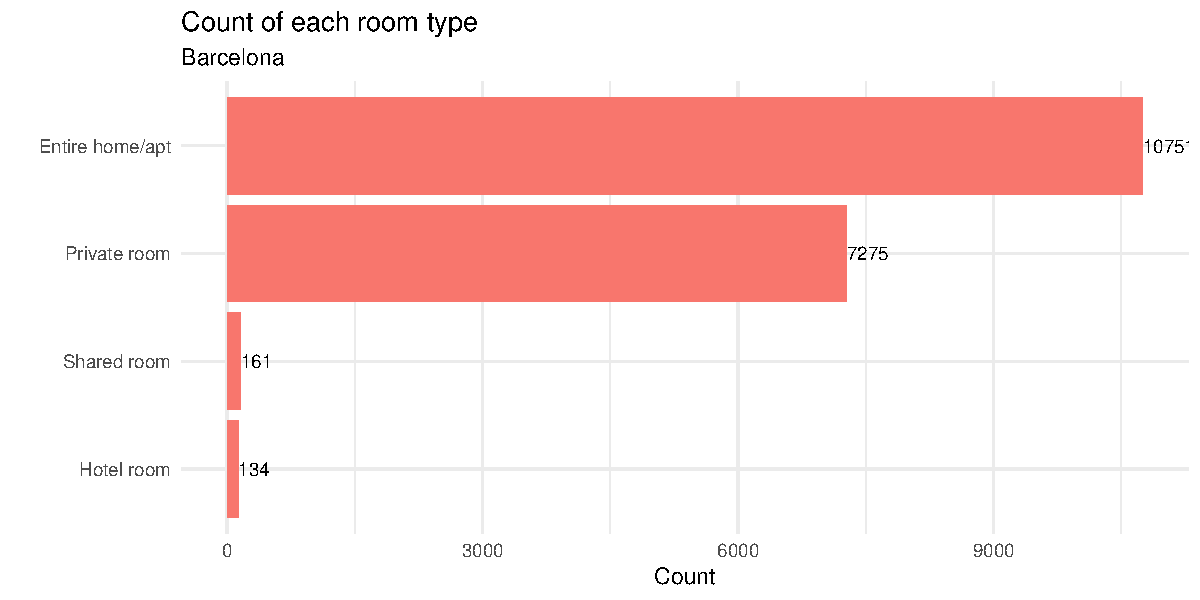
\includegraphics{Barcelona-AirBnB-Insights_files/figure-latex/plot1-1} \end{center}

A straightforward visualization of the dataset's listings already
reveals diverse concentrations, aligning with popular tourist and
overnight stay destinations in Barcelona. The primary cluster is
situated in the expansive neighborhood of \emph{Eixample} and
\emph{Ciutat Vella}, along with \emph{Gràcia}, and the vicinity
encompassing the main train station of \emph{Sants} and \emph{Montjuïc}.
The density significantly diminishes beyond these central regions. It is
essential to acknowledge that the recorded data corresponds to the
official district divisions of Barcelona, delineated by their
boundaries. It is plausible that additional clusters of listings may
exist outside these demarcations. For instance, areas like the proximity
of the airport in the southwestern town of \emph{El Prat de Llobregat}
might host distinct clusters. Incorporating such regions into future
studies could uncover valuable insights in this regard.

\begin{center}\rule{0.5\linewidth}{0.5pt}\end{center}

\hypertarget{airbnb-listings-by-neighbourhood-group}{%
\paragraph{2.3.2. Airbnb listings by neighbourhood
group}\label{airbnb-listings-by-neighbourhood-group}}

\begin{center}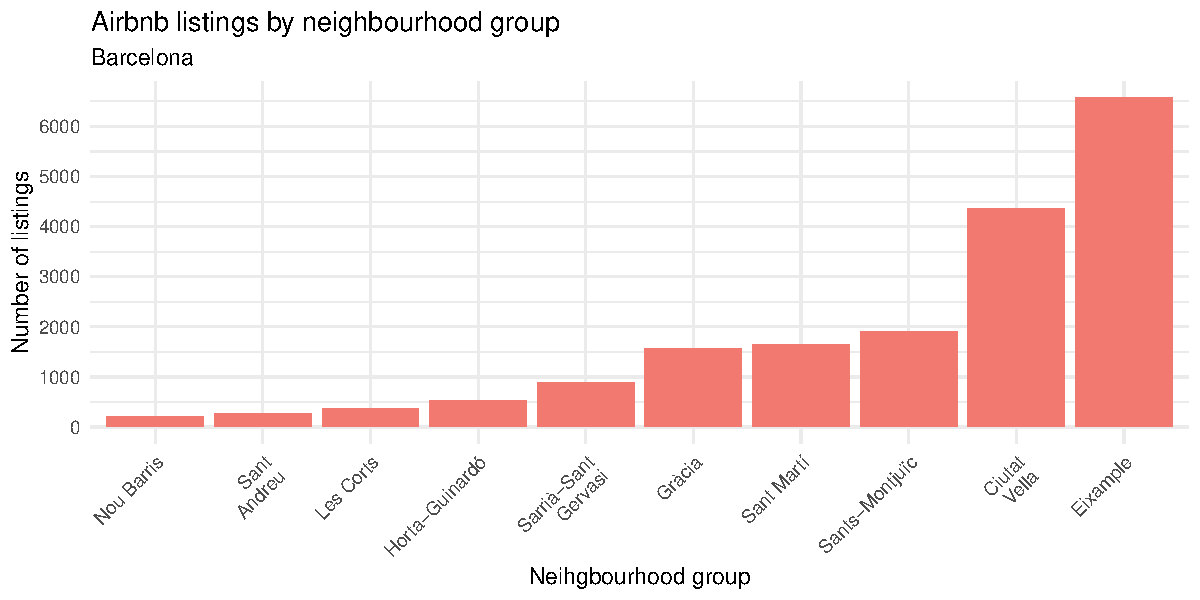
\includegraphics{Barcelona-AirBnB-Insights_files/figure-latex/plot2-1} \end{center}

This bar chart illustrates the number of Airbnb listings across
different neighbourhoods in Barcelona. The most prominent feature is the
overwhelming dominance of the \emph{Eixample} neighbourhood, with the
number of listings towering over other areas. This suggests
\emph{Eixample} is a highly sought-after area for tourists or visitors
using Airbnb. In contrast, neighbourhoods like \emph{Nou Barris} and
\emph{Sant Andreu} have far fewer listings, which may indicate less
tourist activity or a lower availability of rental properties on Airbnb.

The distribution indicates a potential disparity in the spread of
tourism across the city, with certain areas possibly facing higher
pressure from tourist accommodation. It is very interesting to note that
only considering \emph{Eixample} the number of listings is greater than
the sum of the last six neighborhoods. This could have implications for
local housing markets, infrastructure demand, and urban planning. The
chart effectively highlights the disparities and could serve as a basis
for more detailed analysis on the impact of short-term rentals on the
urban landscape of Barcelona. As mentioned, there are several areas that
do not reach a few hundred listings, which indicates a very low
concentration of Airbnbs in relation to the people who reside there.

\begin{center}\rule{0.5\linewidth}{0.5pt}\end{center}

\hypertarget{airbnb-listings-per-100-residents-by-neighbourhood-group}{%
\paragraph{2.3.3. Airbnb listings per 100 residents by neighbourhood
group}\label{airbnb-listings-per-100-residents-by-neighbourhood-group}}

\begin{center}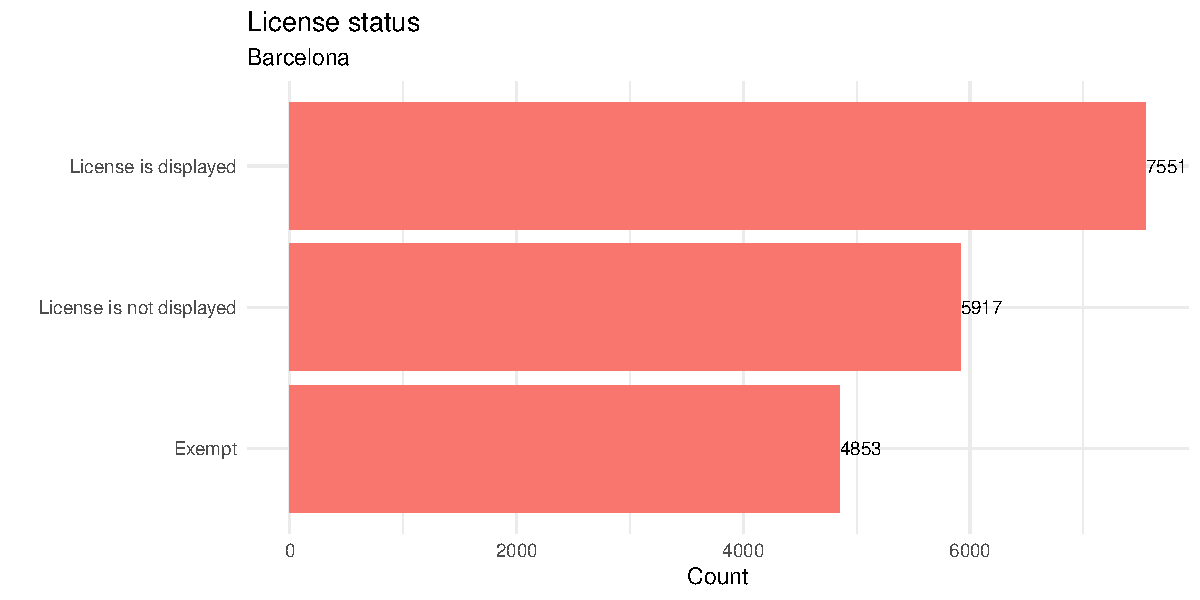
\includegraphics{Barcelona-AirBnB-Insights_files/figure-latex/plot3-1} \end{center}

The data presented in this bar graph serves as an insightful complement
to the previous visualization. By comparing the number of listings in
each neighbourhood group with the official demographics corresponding to
that district, a proportion of Airbnb listings per person can be
obtained. This better reflects the different densities of listings
between parts of the city. Although \emph{Eixample} and \emph{Ciutat
Vella} still reign as the most listing-saturated districts, the higher
concentration of \emph{Ciutat Vella} compared to \emph{Eixample} becomes
obvious. This is explained by many factors, such as the higher urban
density of the Old City and the resulting higher concentration of
population by area, and also \emph{Eixample} being a rather large
district within Barcelona. Similar observations can be made between the
other neighbourhood groups.

According to the
\href{https://web.gencat.cat/es/actualitat/detall/Regulacio-de-pisos-turistics-per-garantir-lacces-a-lhabitatge}{Government
of Catalonia}, areas with more than 5 tourist housing listings per 100
inhabitants face housing access issues. A recent Decree Law has set this
limit to address the problem, with city councils having the authority to
permit up to 10 through their urban planning. It is important to note
that our study focuses exclusively on Airbnb listings, and other units
may be legally listed as tourist accommodations on different platforms.

\begin{center}\rule{0.5\linewidth}{0.5pt}\end{center}

\hypertarget{room-type-count}{%
\paragraph{2.3.4. Room type count}\label{room-type-count}}

\begin{center}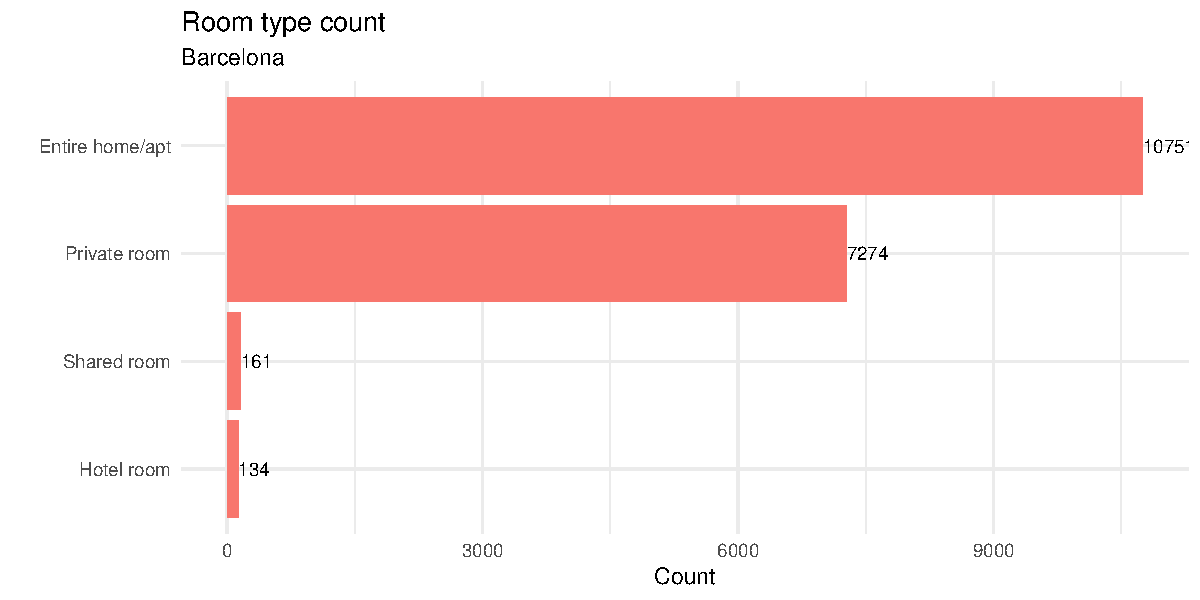
\includegraphics{Barcelona-AirBnB-Insights_files/figure-latex/plot4-1} \end{center}

There are four categories of room types displayed:
\texttt{Entire\ home/apt}, \texttt{Private\ room},
\texttt{Shared\ room}, and \texttt{Hotel\ room}.

The \texttt{Entire\ home/apt} category has the highest count, surpassing
the 10,000 mark, suggesting that entire apartments or homes are the most
common type of property listed in Barcelona. The \texttt{Private\ room}
category follows, with roughly half as many listings as entire homes,
indicating a significant presence in the market but less than the full
property rentals.

\texttt{Shared\ rooms} and \texttt{Hotel\ rooms} have significantly
fewer listings compared to the other two categories. Shared rooms barely
register on the scale, suggesting they are a less popular option among
the listings. Hotel rooms have the smallest count, indicating that
traditional hotel stays are much less commonly listed on platforms
likely compared to short-term rental options.

The visual emphasizes the prevalence of whole property rentals in
Barcelona's accommodation offerings, with a substantial secondary market
for private rooms. The minimal presence of shared and hotel room
listings could reflect market demand or possibly restrictions and
regulations within the city.

\begin{center}\rule{0.5\linewidth}{0.5pt}\end{center}

\hypertarget{acommodation-type-by-neighbourhood-group}{%
\paragraph{2.3.5. Acommodation type by neighbourhood
group}\label{acommodation-type-by-neighbourhood-group}}

\begin{center}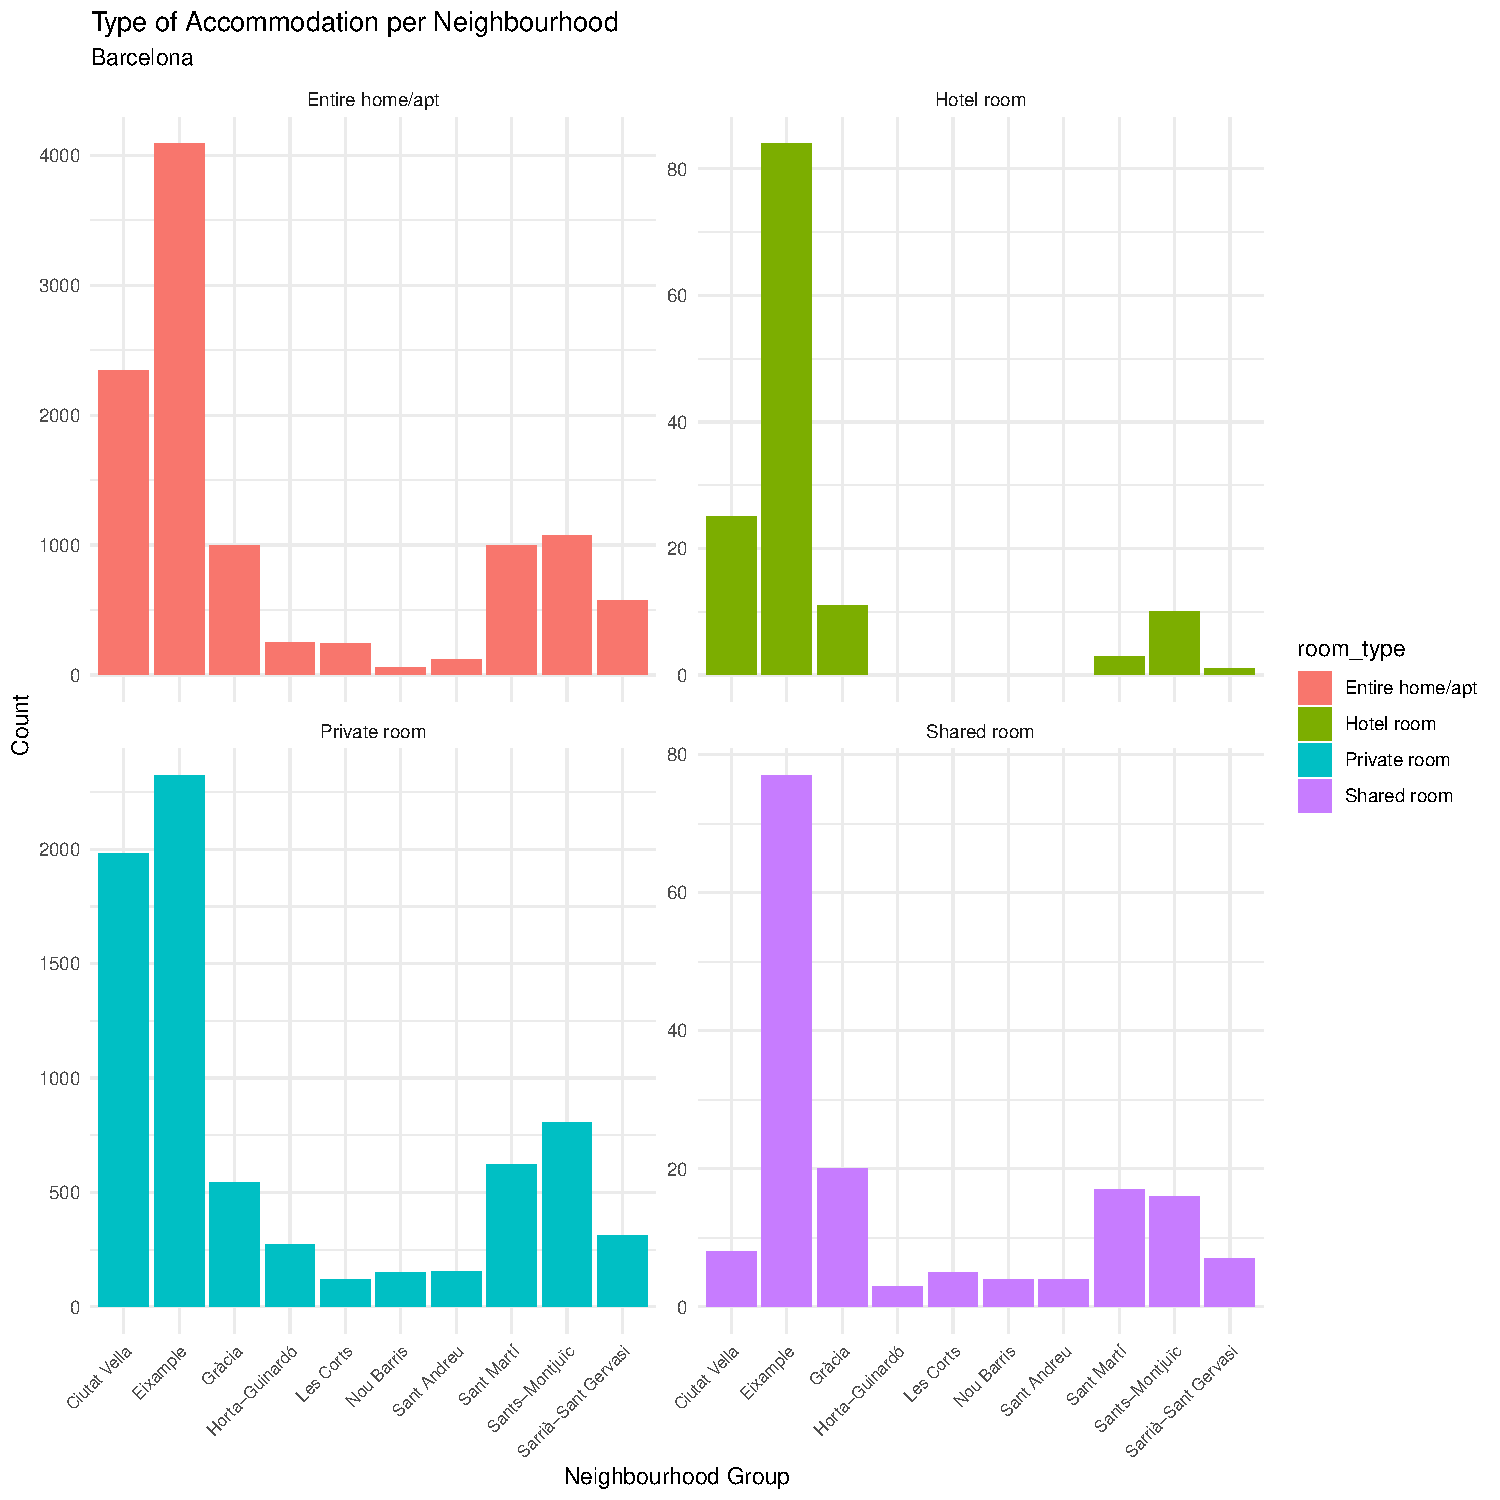
\includegraphics{Barcelona-AirBnB-Insights_files/figure-latex/plot5-1} \end{center}

This chart provides a detailed breakdown of Airbnb listings in Barcelona
by room type and neighbourhood group, with four distinct categories of
accommodation: \texttt{entire\ home/apt}, \texttt{hotel\ room},
\texttt{private\ room}, and \texttt{shared\ room}. The y-axis represents
the number of listings, which is not consistent across the categories,
indicating the use of a free scale within the facets to better display
the range of data.

\begin{itemize}
\item
  Focusing first on the \texttt{Entire\ home/apt} category, we observe a
  pronounced peak in \emph{Eixample}, with over 4,000 listings, which
  significantly overshadows the counts in other areas, where the
  second-highest listing \emph{Ciutat Vella} has just above 1,000. This
  indicates a heavy concentration of full-property rentals in that
  particular part of the city, which shows that \emph{Eixample} is a
  popular central area known for tourist attractions.
\item
  The \texttt{Hotel\ room} category exhibits a very different scale,
  peaking at around 80 listings in the most prominent neighbourhood,
  being again \emph{Eixample} for this category. This suggests that
  hotel rooms are a minor part of the Airbnb market in Barcelona or that
  hotels prefer to use other channels for renting out rooms. There are
  several neighborhoods that do not even present a single hotel listing.
\item
  For \texttt{Private\ rooms}, the distribution seems more even, yet
  \emph{Eixample} stands out with nearly 2,000 listings, which is about
  triple the number of listings in the second next populous neighborhood
  in this category, \emph{Sants-Montjuïc}. The shape of the graph is
  surprisingly similar to the \texttt{Entire\ home/apt}.
\item
  The \texttt{Shared\ room} type displays the least number of listings
  across neighborhoods, with the highest being under 80. The low count
  could indicate that shared rooms are not a preferred choice for
  visitors to Barcelona, or such listings are rare.
\end{itemize}

The vast discrepancy between the number of \texttt{Entire\ home/apt}
listings and other types suggests that visitors to Barcelona may prefer
the privacy and space of an entire apartment. The data could also imply
a potential regulatory environment that either supports whole-home
rentals or one that has yet to address this preference in the sharing
economy.

The chart is an excellent tool for stakeholders to assess market
saturation in various neighborhoods and room types. For investors and
property managers, areas with lower counts could represent potential
growth opportunities. Conversely, neighborhoods with high listings might
face more competition, affecting pricing strategies. For policymakers
such as OMIC and the Barcelona City hall, such data can be crucial in
understanding how short-term rentals are distributed across the city and
may guide decisions on tourism management, zoning, and housing policies
to balance the needs of residents and visitors.

\begin{center}\rule{0.5\linewidth}{0.5pt}\end{center}

\hypertarget{license-status-1}{%
\paragraph{2.3.6. License status}\label{license-status-1}}

\begin{center}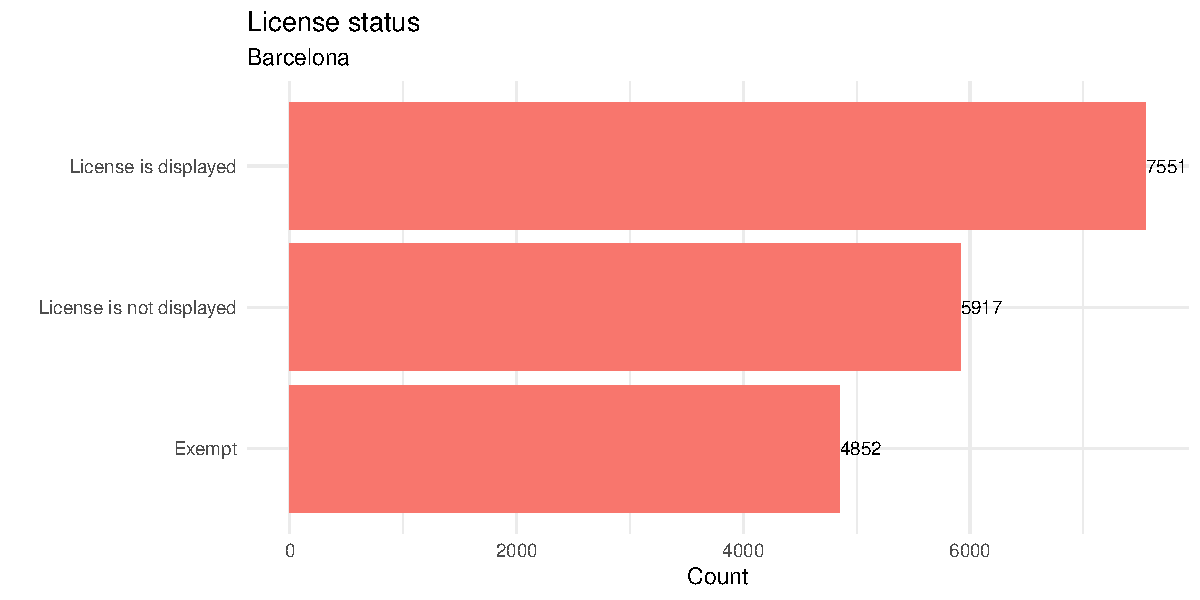
\includegraphics{Barcelona-AirBnB-Insights_files/figure-latex/plot6-1} \end{center}

This visualization provides a rough insight into the licensing status of
listings. According to the law, full-home listings require a
registration and a license number. Instances under the
\texttt{License\ not\ displayed} group may either be listed illegally or
have their license approval pending. \texttt{Exempt} could mean a
listing only includes part of a housing unit or a room, and thus does
not have to be legally registered as full touristic housing. It would be
valuable to observe the evolution of the \texttt{License\ is\ displayed}
group over time, to evaluate whether the city's efforts to regulate
touristic housing have any effectiveness.

\begin{center}\rule{0.5\linewidth}{0.5pt}\end{center}

\hypertarget{large-vs.-small-tenants}{%
\paragraph{2.3.7. Large vs.~small
tenants}\label{large-vs.-small-tenants}}

\begin{center}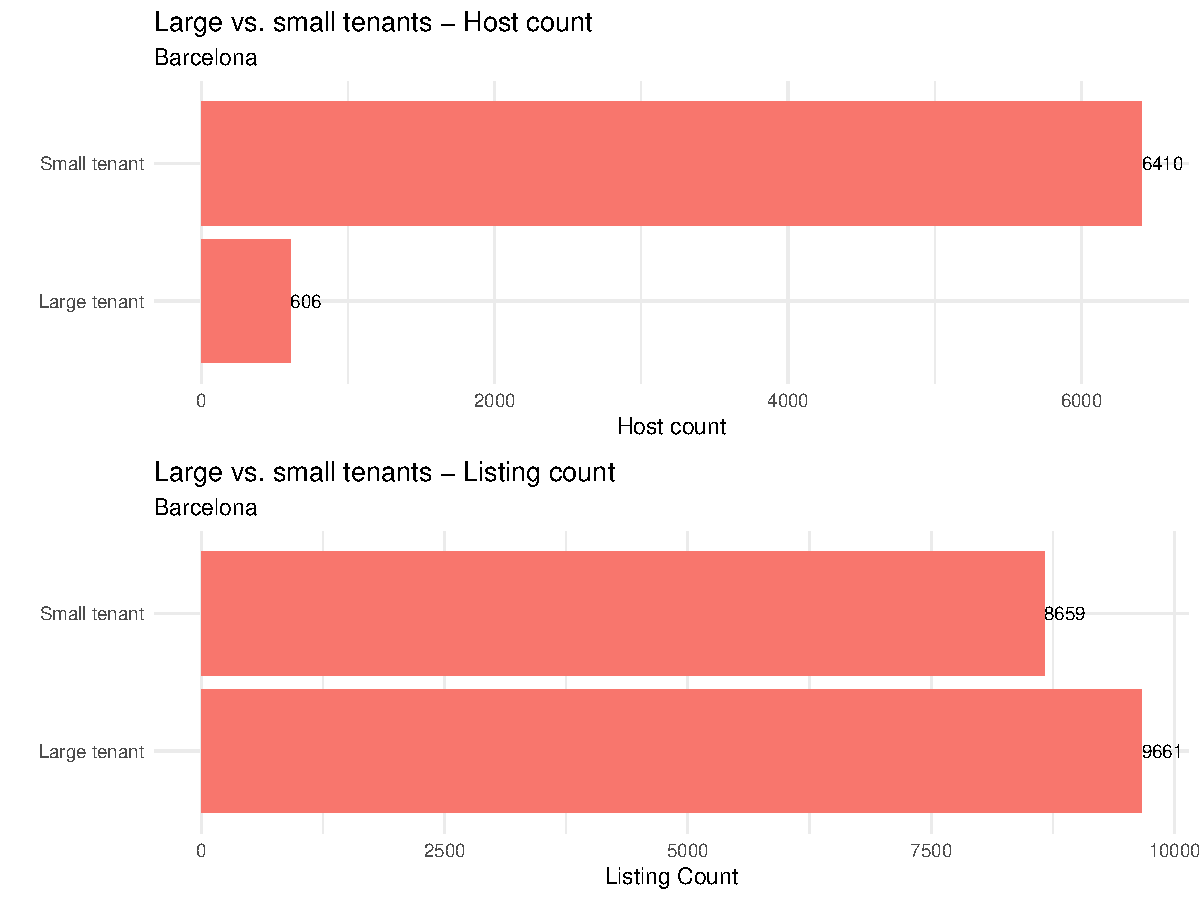
\includegraphics{Barcelona-AirBnB-Insights_files/figure-latex/plot7-1} \end{center}

This set of charts looks at two host categories: \texttt{Small\ tenant}
and \texttt{Large\ tenant}, based on the number of listings they
possess. Given the context of rental tension zones, a
\href{https://www.boe.es/buscar/act.php?id=BOE-A-2023-12203}{recent
legislation} changed the definition of a large property owner from 10 to
5 properties. This meant that several former small tenants now qualify
as large tenants, potentially altering the market dynamics and affecting
the application of policies within stressed areas.

In the first plot, the count of \texttt{Small\ tenant} vastly outnumbers
\texttt{Large\ tenant}, indicating a much higher proportion of landlords
with fewer properties. This however is reflected otherwise when looking
at the overall \texttt{Listing\ count} in the second plot, which shows a
very close match between number of listings that are registered by
\texttt{Small\ tenant} and \texttt{Large\ tenant}.

From this observation we can conclude that, although much fewer in
number, large tenants represent the majority of the overall market. It
is also worth noting that the presence of more small tenants could
reflect a diverse range of property offerings, from single rooms to
entire apartments, which may cater to different segments of the
population. This might have a stabilizing effect on rental prices, as a
diverse supply can meet varied demand. However, if small tenants begin
to consolidate or if their listings push housing costs above the 30\%
income threshold, it could lead to increased regulatory scrutiny.

Regarding the law's stipulations, if the large tenants' listings are
concentrated in areas where housing costs exceed 30\% of household
income or where rental prices have outpaced CPI by more than 3
percentage points, these areas could be designated as rental tension
zones. This would trigger regulatory measures that could include rent
capping or other controls to protect tenants.

\begin{center}\rule{0.5\linewidth}{0.5pt}\end{center}

\hypertarget{number-of-hosts-per-listing-count}{%
\paragraph{2.3.8. Number of hosts per listing
count}\label{number-of-hosts-per-listing-count}}

\begin{center}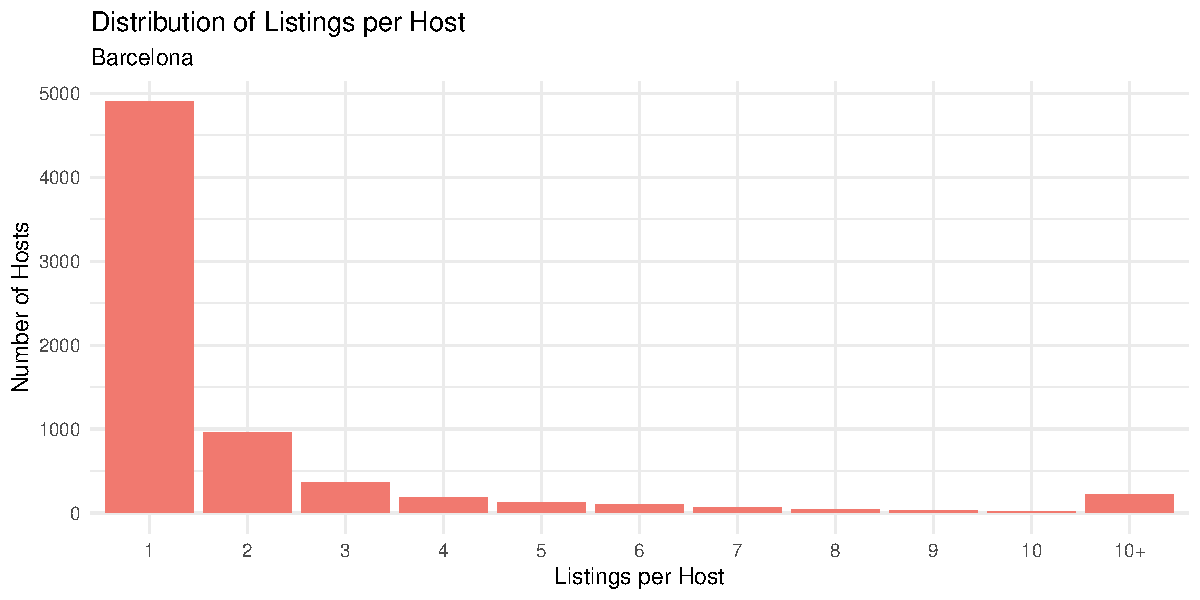
\includegraphics{Barcelona-AirBnB-Insights_files/figure-latex/plot8-1} \end{center}

The above plot illustrates another defining observation, by sorting all
Airbnb hosts according to the number of listings they have registered on
the platform. Represented in the variable \texttt{Number\ of\ hosts},
out of a total of 7,015 hosts, an overwhelming majority is responsible
for only one listing, with a quick decrease in number as the
\texttt{Listing\ count} increases

It becomes obvious that the market is overwhelmingly populated by
1-property hosts, suggesting a high level of competitiveness and
relatively low monopoly of the market

\begin{center}\rule{0.5\linewidth}{0.5pt}\end{center}

\hypertarget{top-5-hosts-by-number-of-listings}{%
\paragraph{2.3.9. Top 5 hosts by number of
listings}\label{top-5-hosts-by-number-of-listings}}

\begin{center}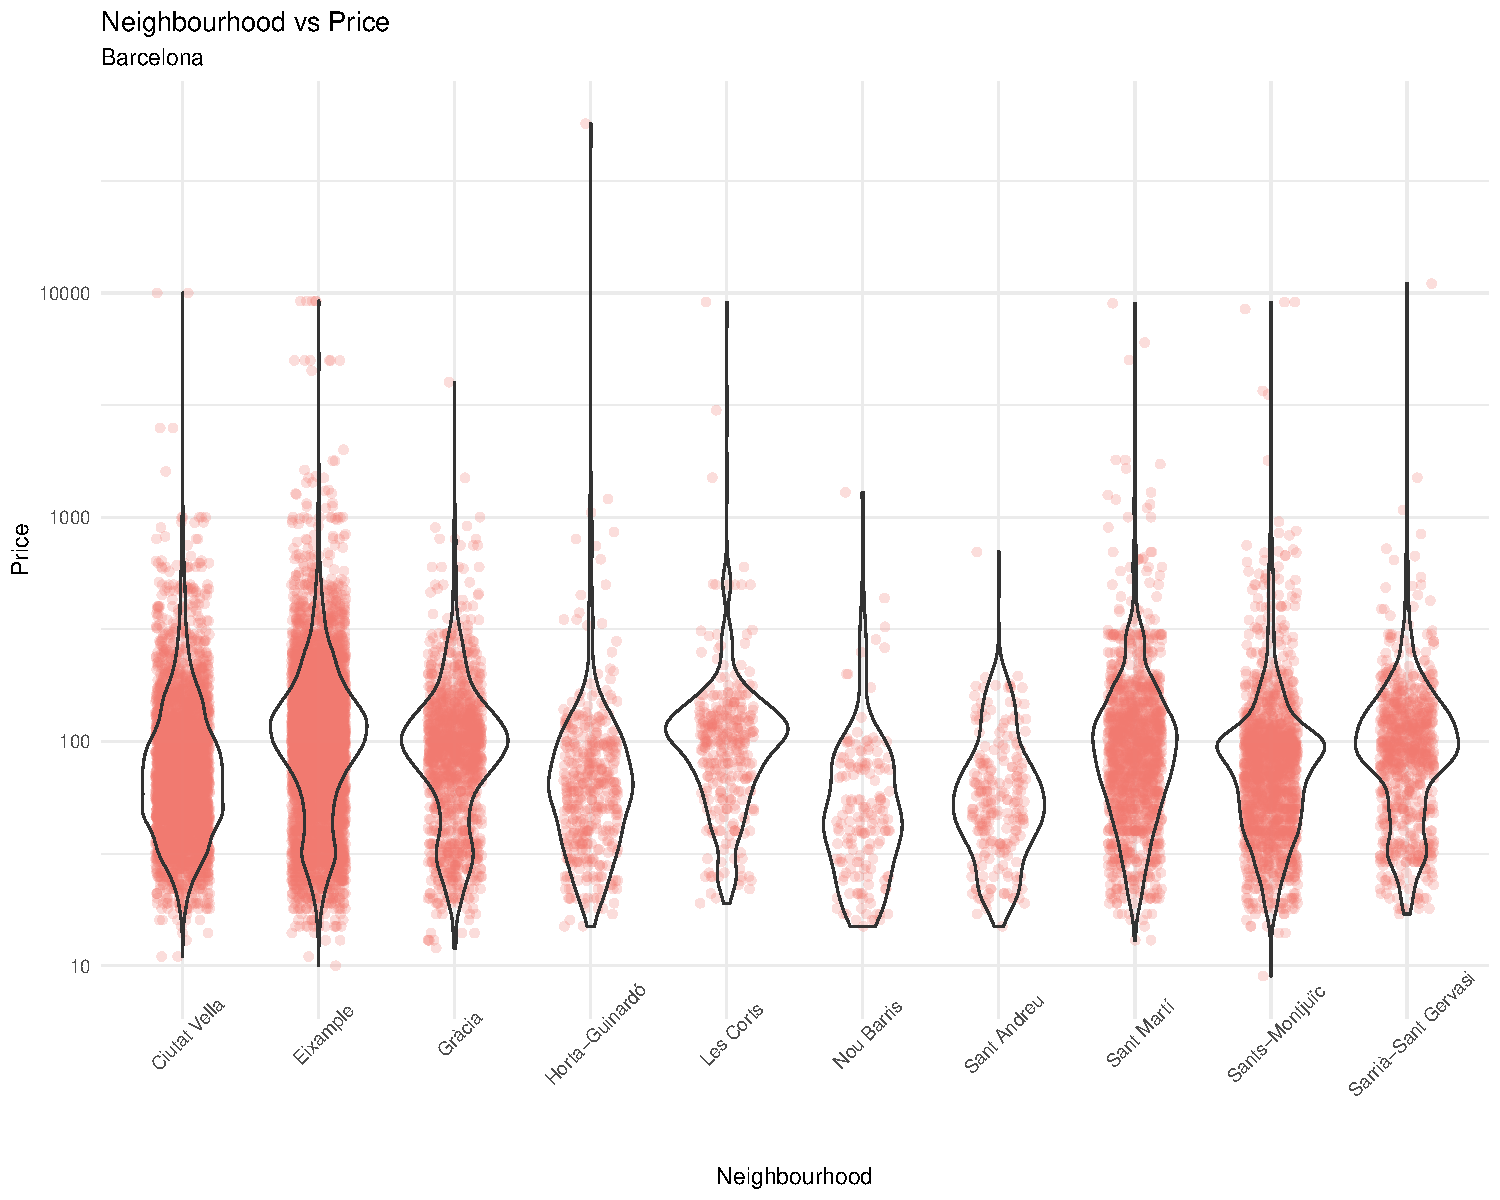
\includegraphics{Barcelona-AirBnB-Insights_files/figure-latex/plot9-1} \end{center}

To provide further insight into the host number and listing count
disparity, by querying through unique items of \texttt{host\_id}, and
sorting based on \texttt{calculated\_host\_listings\_count} we can
obtain the 5 top hosts by number of listings. A brief look at the graph
reveals that each of the five entities is accountable for a
significantly greater number of properties than what is deemed as
characteristic of large tenants according to the law. Also, the
assumption could be made that the names reflect that such hosts are not
actual individual human users of the platform, but rather companies or
trusts, which operate large touristic housing rental businesses across
Barcelona.

\begin{center}\rule{0.5\linewidth}{0.5pt}\end{center}

\hypertarget{average-price-by-neighbourhood}{%
\paragraph{2.3.10. Average price by
neighbourhood}\label{average-price-by-neighbourhood}}

\begin{center}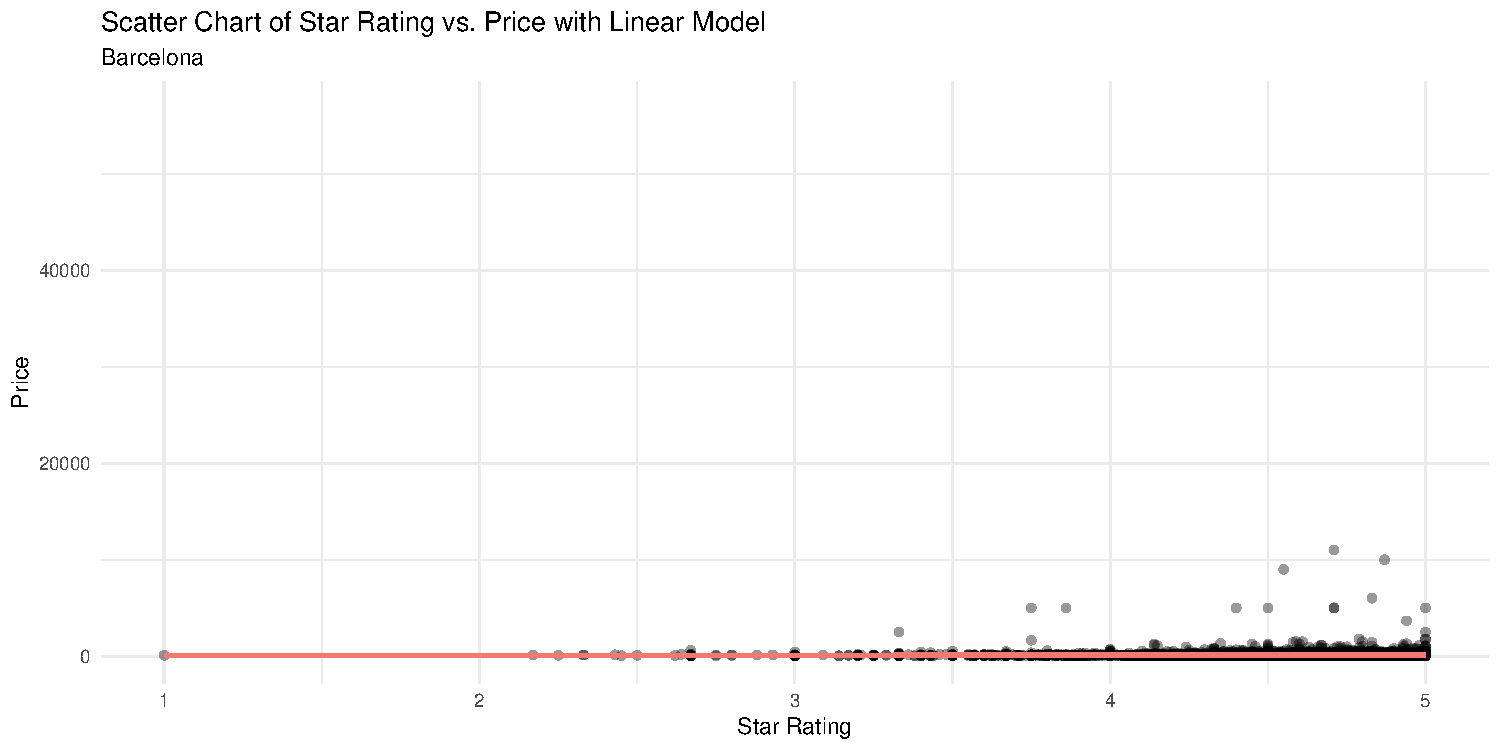
\includegraphics{Barcelona-AirBnB-Insights_files/figure-latex/plot10-1} \end{center}

The map above illustrates the districts of Barcelona (the 71 divisions
designated by the City Council), with colors representing a gradient
based on the average price of Airbnb listings in each area. The average
prices range from approximately €50 to €250, revealing a general trend
of decreasing prices in neighborhoods farther from the center and
popular districts, with a subtle decline from south to north. However,
this pattern is disrupted by stark outliers, notably in the
neighborhoods of \emph{Sant Gervasi - la Bonanova} and \emph{la
Maternitat i Sant Ramon}. These anomalies can be attributed to a few
exclusive listings in the vicinity of €10,000 per night. The reason for
these extremes may be the unique nature of these listings as highly
exclusive overnight units, such as villas or large fully furnished
houses, or also potential data quality issues. As this report focuses
solely on observations, a more in-depth analysis of these factors would
be suitable for a future iteration of the study.

\begin{center}\rule{0.5\linewidth}{0.5pt}\end{center}

\hypertarget{price-by-neighbourhood-group}{%
\paragraph{2.3.11. Price by neighbourhood
group}\label{price-by-neighbourhood-group}}

\begin{center}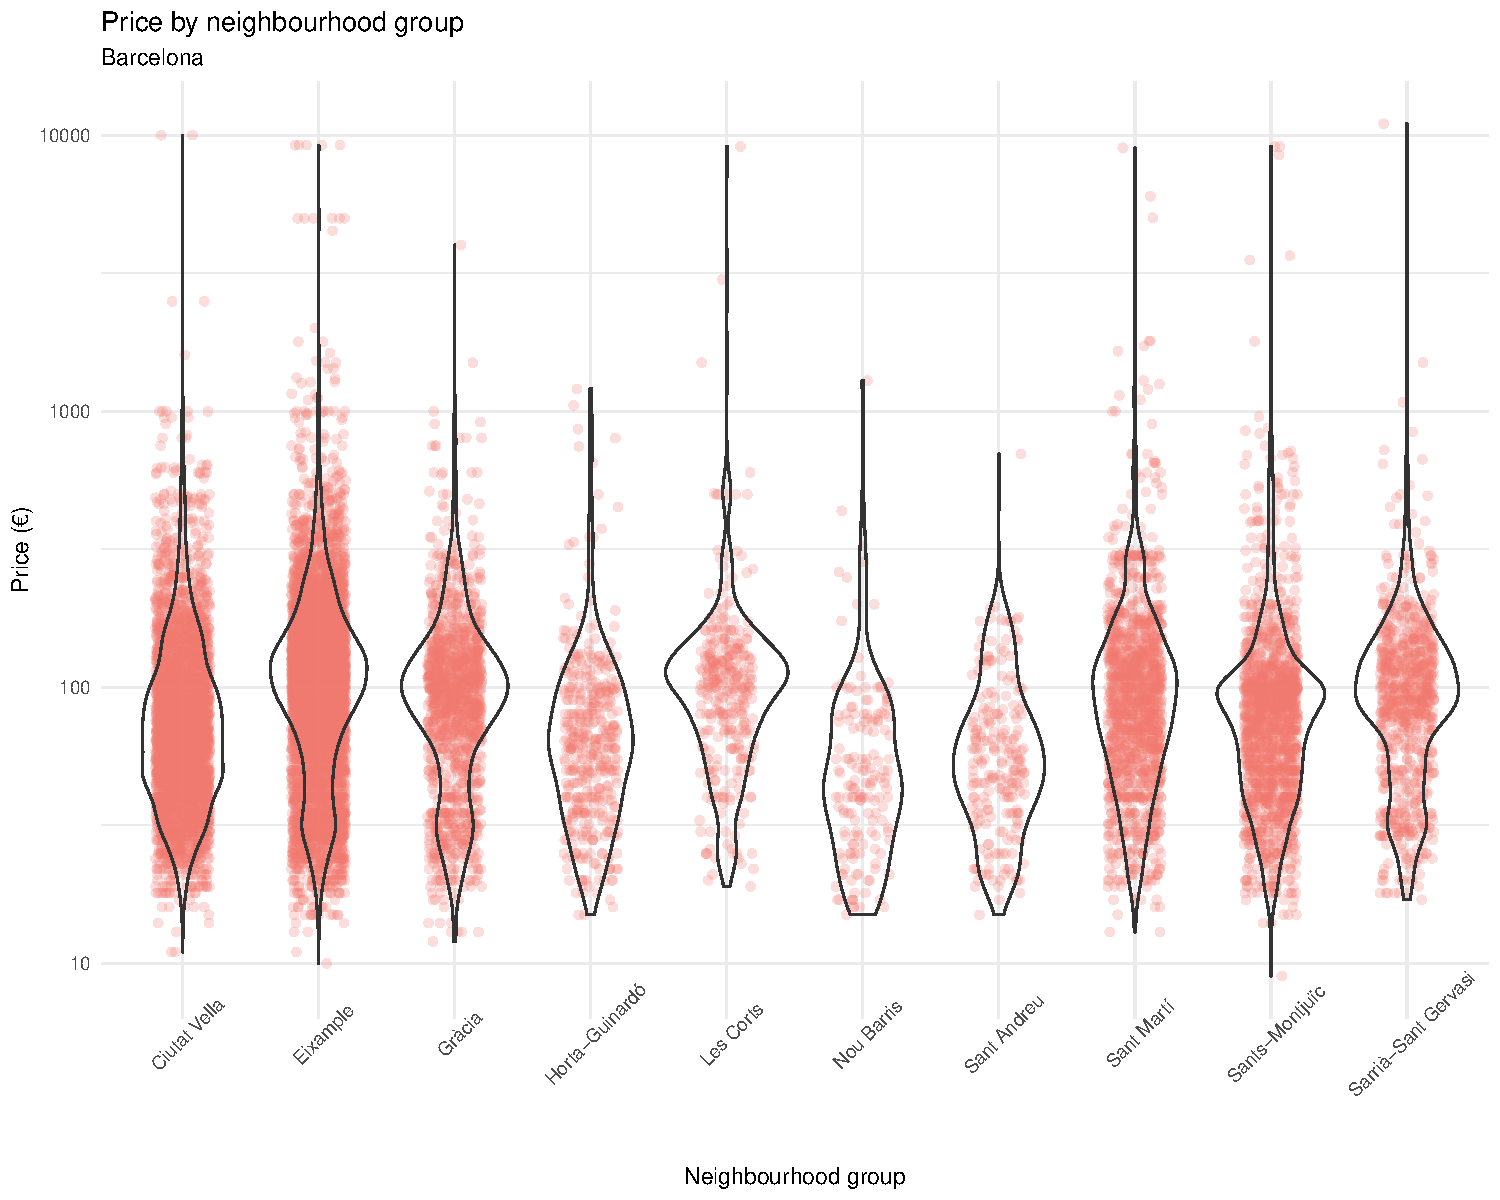
\includegraphics{Barcelona-AirBnB-Insights_files/figure-latex/plot11-1} \end{center}

This plot provides some further insight into the distribution of the
\texttt{price} variable that is not conveyed in the previous map plot.
The \texttt{price} of listings is represented as points on a scatter
plot, and clustered by \texttt{neighbourhood\_group} in order to reflect
the actual variation of values, and locate the \emph{center} of the
distributions. Because most listings' \texttt{price} values are located
around the €100 range (median is €87), the items with much higher
pricing significantly skew the plot. Thus, in order to improve the
readability of the \emph{median region}, the scale has been adjusted to
be logarithmic. The additional violin plot lines provide more
information about the distribution and location of medians.

Corroborating observations from previous graphs, the majority of
listings is seen to concentrate in the \emph{Ciutat Vella} and
\emph{Eixample} districts, with the latter containing the highest
median, as well as highest listing count, of all districts. On the other
hand, the furthest-located districts of \emph{Nou Barris} and \emph{Sant
Andreu} are seen to contain the least and overall lowest-priced listings
of the city.

\begin{center}\rule{0.5\linewidth}{0.5pt}\end{center}

\hypertarget{price-boxplots-by-neighbourhood-group}{%
\paragraph{2.3.12. Price boxplots by neighbourhood
group}\label{price-boxplots-by-neighbourhood-group}}

\begin{center}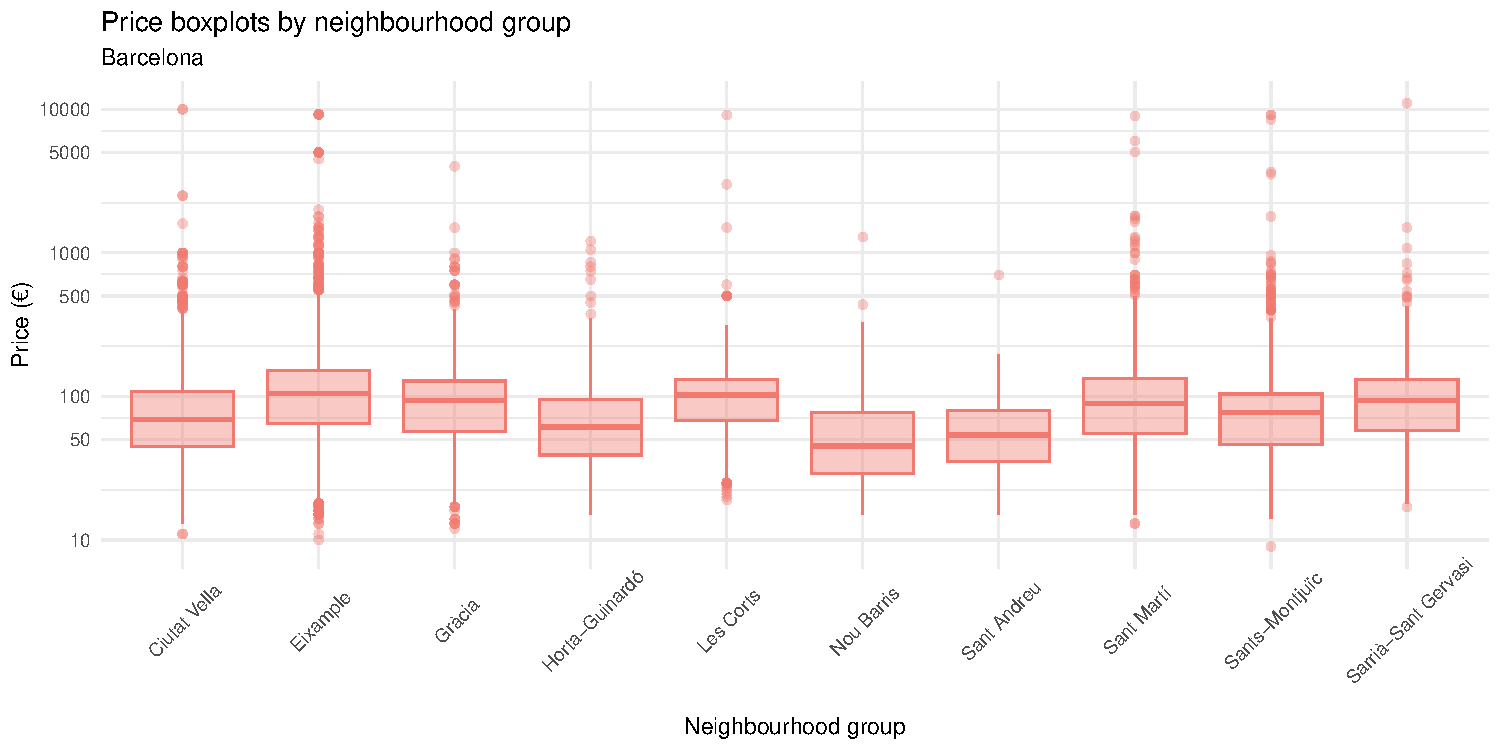
\includegraphics{Barcelona-AirBnB-Insights_files/figure-latex/plot12-1} \end{center}

The previous plot could be summarized in the above boxplot, which
locates the quartiles and medians for the \texttt{price} variable in
each neighbourhood group. As an example, the following are the medians
from the neighbourhood groups mentioned in the previous plot, which
represent the lowest and highest extremes in all 10:

\begin{Shaded}
\begin{Highlighting}[]
\FunctionTok{median}\NormalTok{(Barcelona\_md}\SpecialCharTok{$}\NormalTok{price[Barcelona\_md}\SpecialCharTok{$}\NormalTok{neighbourhood\_group }\SpecialCharTok{==} \StringTok{"Ciutat Vella"}\NormalTok{], }\AttributeTok{na.rm =} \ConstantTok{TRUE}\NormalTok{)}
\end{Highlighting}
\end{Shaded}

\begin{verbatim}
## [1] 69
\end{verbatim}

\begin{Shaded}
\begin{Highlighting}[]
\FunctionTok{median}\NormalTok{(Barcelona\_md}\SpecialCharTok{$}\NormalTok{price[Barcelona\_md}\SpecialCharTok{$}\NormalTok{neighbourhood\_group }\SpecialCharTok{==} \StringTok{"Eixample"}\NormalTok{], }\AttributeTok{na.rm =} \ConstantTok{TRUE}\NormalTok{)}
\end{Highlighting}
\end{Shaded}

\begin{verbatim}
## [1] 105
\end{verbatim}

\begin{Shaded}
\begin{Highlighting}[]
\FunctionTok{median}\NormalTok{(Barcelona\_md}\SpecialCharTok{$}\NormalTok{price[Barcelona\_md}\SpecialCharTok{$}\NormalTok{neighbourhood\_group }\SpecialCharTok{==} \StringTok{"Nou Barris"}\NormalTok{], }\AttributeTok{na.rm =} \ConstantTok{TRUE}\NormalTok{)}
\end{Highlighting}
\end{Shaded}

\begin{verbatim}
## [1] 45
\end{verbatim}

\begin{Shaded}
\begin{Highlighting}[]
\FunctionTok{median}\NormalTok{(Barcelona\_md}\SpecialCharTok{$}\NormalTok{price[Barcelona\_md}\SpecialCharTok{$}\NormalTok{neighbourhood\_group }\SpecialCharTok{==} \StringTok{"Sant Andreu"}\NormalTok{], }\AttributeTok{na.rm =} \ConstantTok{TRUE}\NormalTok{)}
\end{Highlighting}
\end{Shaded}

\begin{verbatim}
## [1] 54
\end{verbatim}

\begin{center}\rule{0.5\linewidth}{0.5pt}\end{center}

\hypertarget{listings-by-minimum-nights}{%
\paragraph{2.3.13. Listings by minimum
nights}\label{listings-by-minimum-nights}}

\begin{center}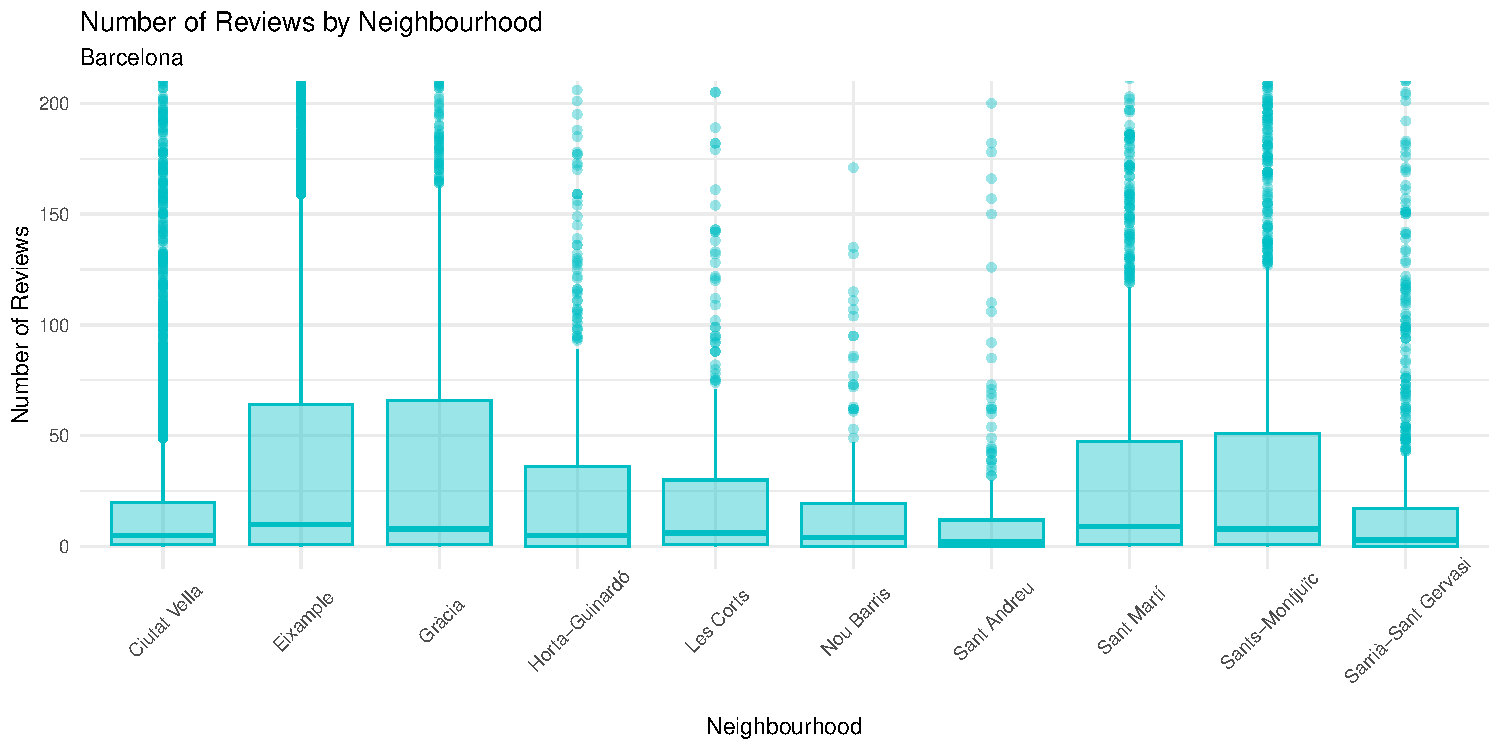
\includegraphics{Barcelona-AirBnB-Insights_files/figure-latex/plot13-1} \end{center}

This chart examines the distribution of listing counts based on the
minimum nights required, aiming to illustrate this variable throughout
the entire dataset. An initial observation can be made that the majority
of listings require a minimum reservation of one night, followed by a
rapid decline in frequency until reaching a full week. Further on, a
significant upsurge in listings happens around the 30-day mark,
indicating that a substantial cluster of listings entail a minimum stay
of around a month.

Such findings lend support to the argument that Airbnb serves as a
portal for an increasingly diverse range of rental types, extending
beyond the original notion of short-term single-room leases, which were
the original hallmark of the platform.

\begin{center}\rule{0.5\linewidth}{0.5pt}\end{center}

\hypertarget{minimum-nights-boxplots-by-neighbourhood-group}{%
\paragraph{2.3.14. Minimum nights boxplots by neighbourhood
group}\label{minimum-nights-boxplots-by-neighbourhood-group}}

\begin{center}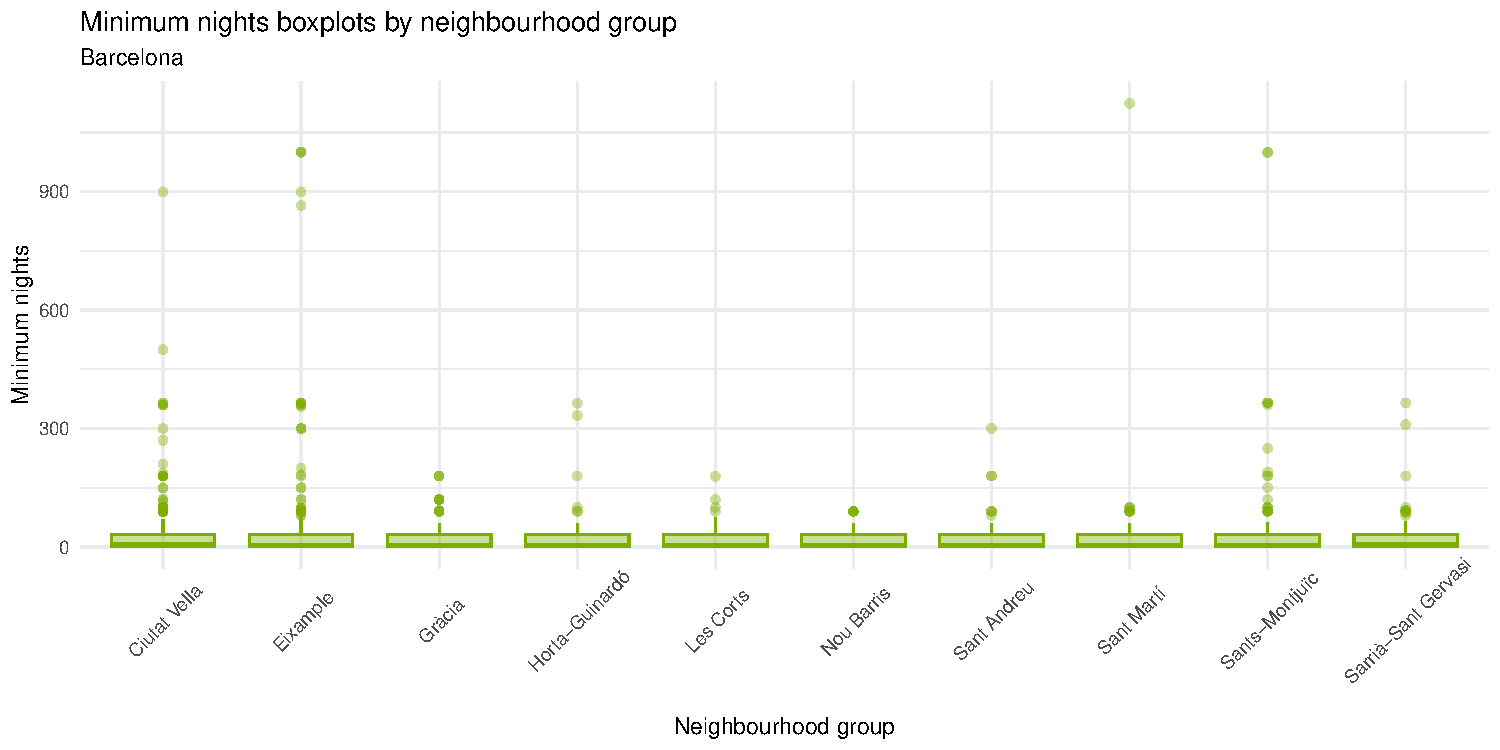
\includegraphics{Barcelona-AirBnB-Insights_files/figure-latex/plot14-1} \end{center}

\begin{center}\rule{0.5\linewidth}{0.5pt}\end{center}

\hypertarget{reviews-boxplots-by-neighbourhood-group}{%
\paragraph{2.3.15. Reviews boxplots by neighbourhood
group}\label{reviews-boxplots-by-neighbourhood-group}}

\begin{center}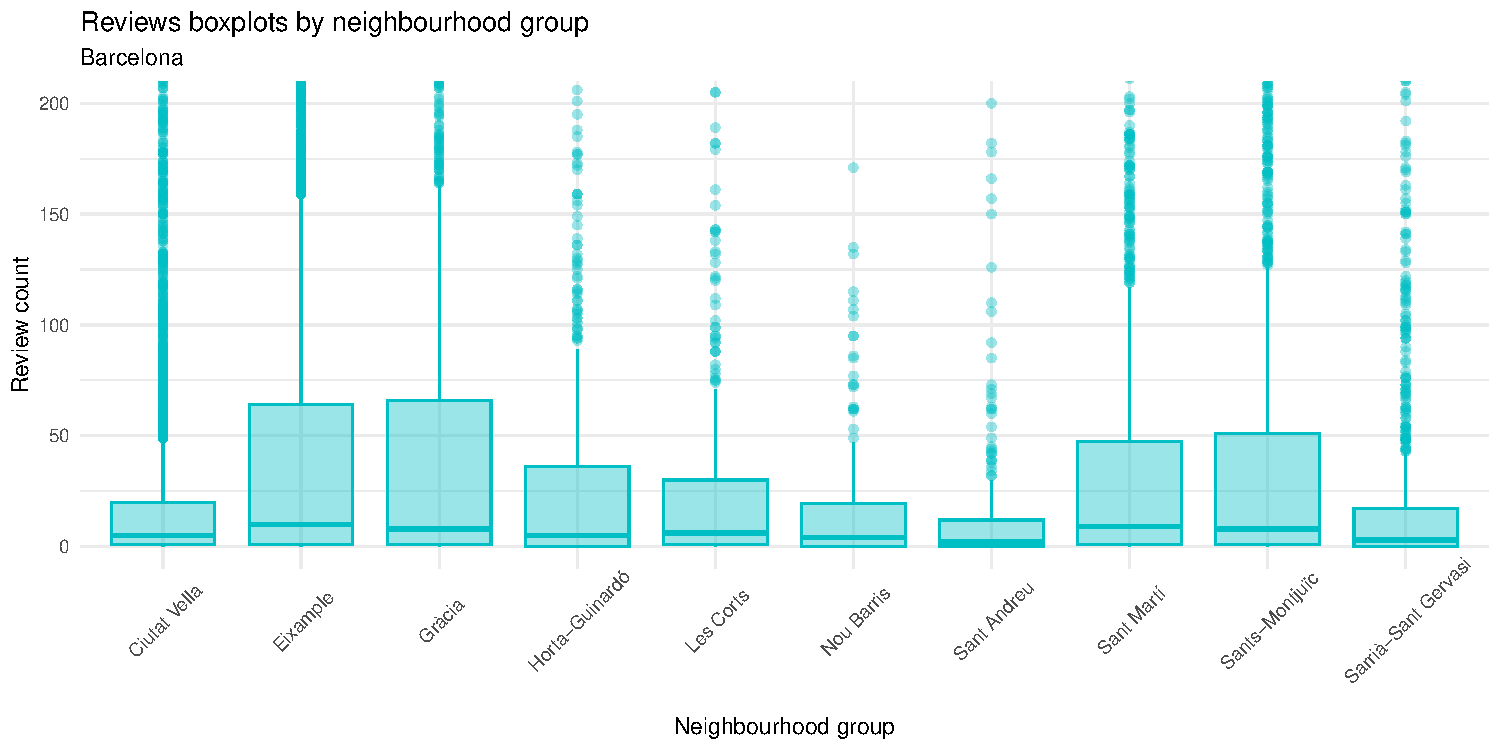
\includegraphics{Barcelona-AirBnB-Insights_files/figure-latex/plot15-1} \end{center}

\begin{center}\rule{0.5\linewidth}{0.5pt}\end{center}

\hypertarget{correlation-of-numerical-values}{%
\paragraph{2.3.16. Correlation of numerical
values}\label{correlation-of-numerical-values}}

\begin{center}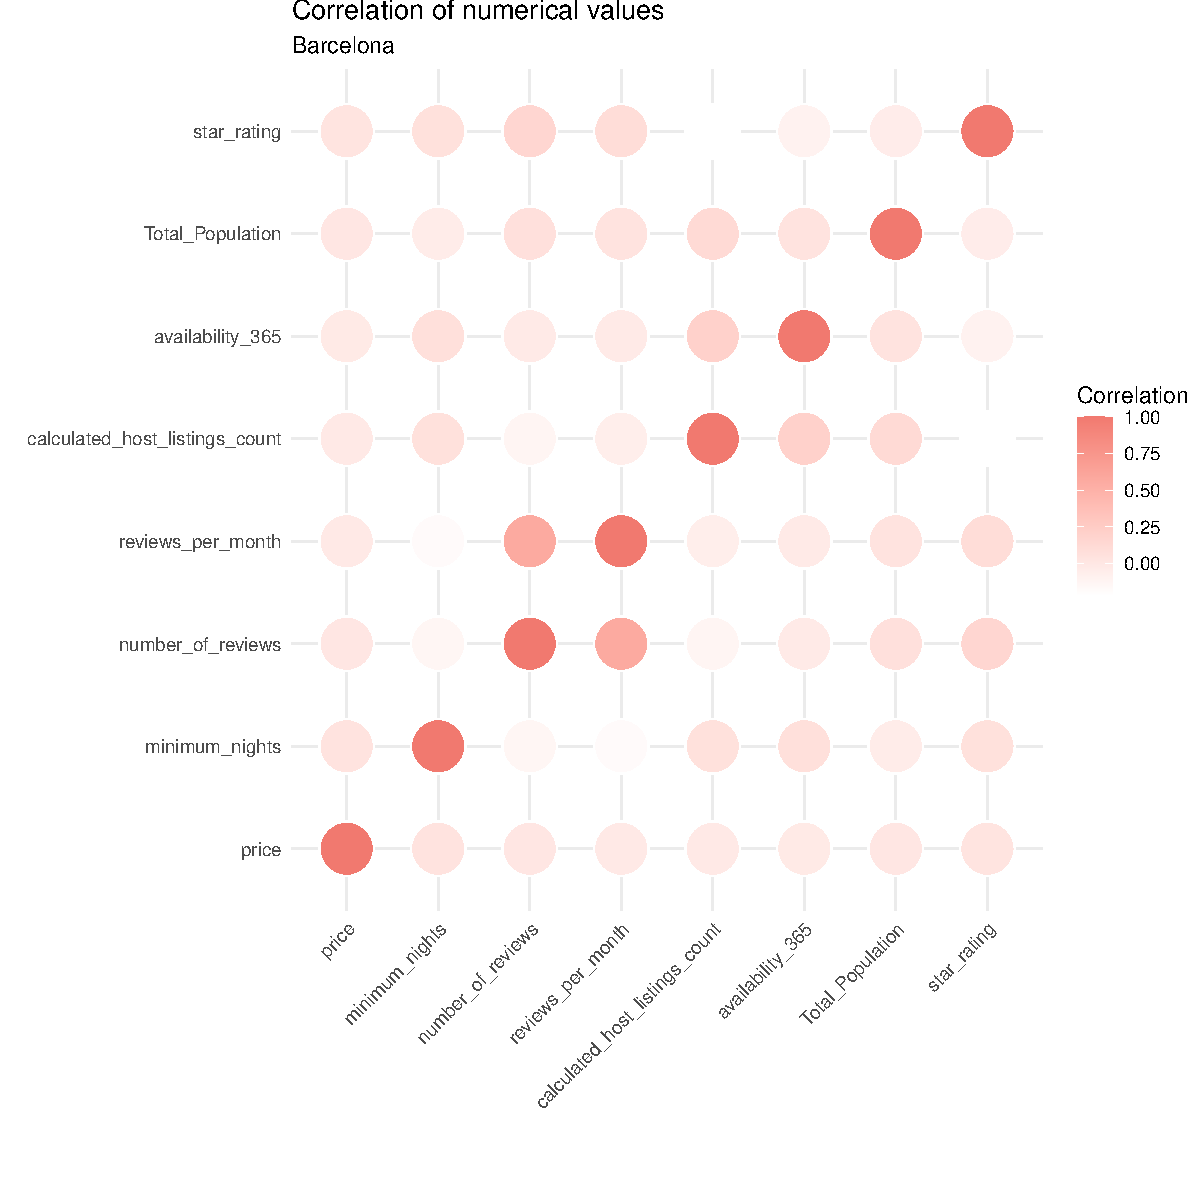
\includegraphics{Barcelona-AirBnB-Insights_files/figure-latex/plot16-1} \end{center}

\begin{center}\rule{0.5\linewidth}{0.5pt}\end{center}

\hypertarget{price-by-star-rating}{%
\paragraph{2.3.17. Price by star rating}\label{price-by-star-rating}}

\begin{center}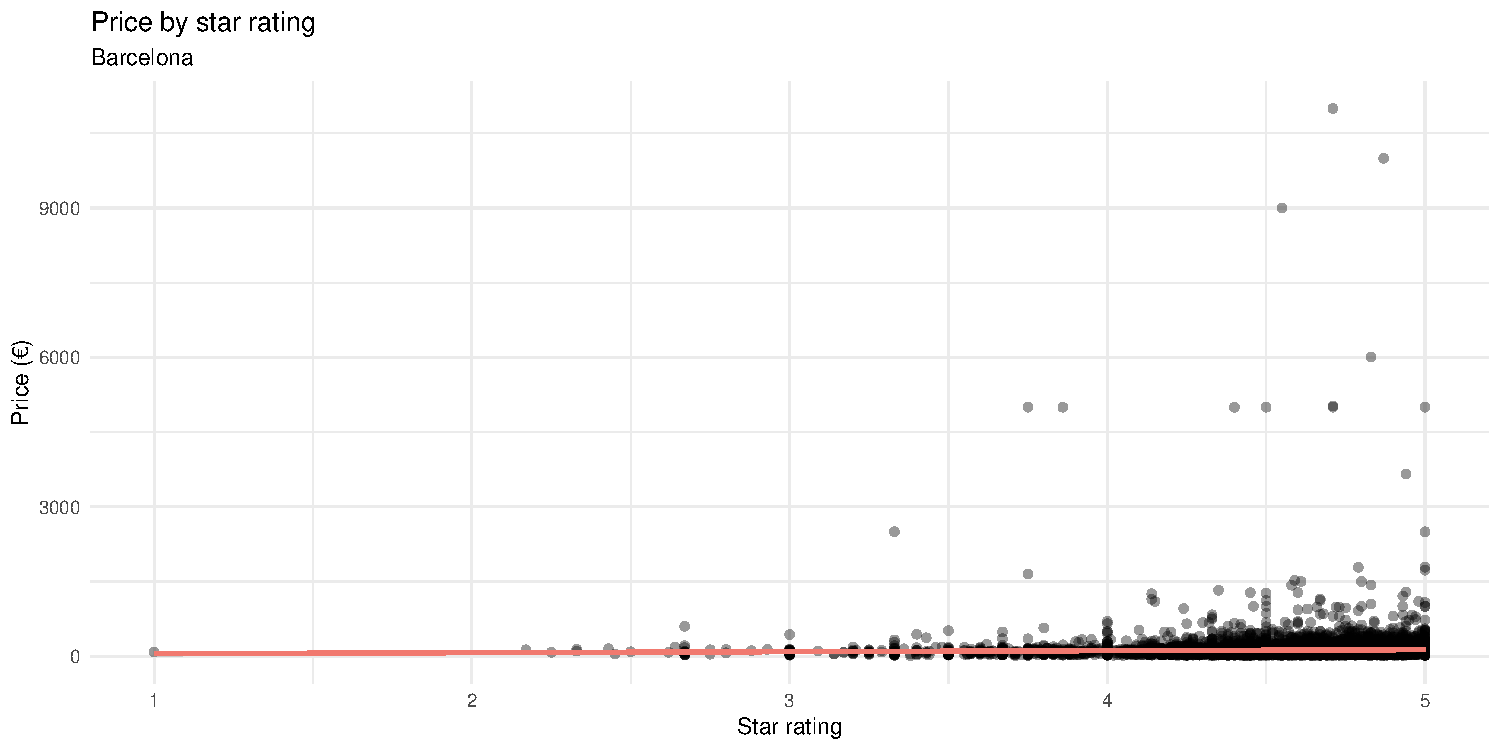
\includegraphics{Barcelona-AirBnB-Insights_files/figure-latex/plot17-1} \end{center}

\begin{center}\rule{0.5\linewidth}{0.5pt}\end{center}

\hypertarget{additional-chapter}{%
\subsection{3. Additional chapter}\label{additional-chapter}}

An additional segment of the project worthy of mention are the
alternative workflows and R packages that we explored, discarded or
eventually implemented into our work.

One notable case was opur strategy for accessing the Open Data BCN
demographics data set, which relied on the Barcelona City Council's API.
We opted for this path with the sole purpose of exploring alternative
data loading workflows, despite the straightforward alternative of
downloading and loading the \texttt{2023\_pad\_mdbas\_sexe.csv} file
from the website being more easily available.

Among other libraries that weren't covered during the Bootcamp, we
incorporated the \texttt{gridExtra} library to manipulate the
\texttt{ggplot2} layout, allowing for efficient division and arrangement
of layouts to optimize visualization.

For the `Average price by neighbourhood' plot (number 10), the package
\texttt{ggrepel} was tested and loaded in order to position the labels
for the neighbourhood polygons in such a way that they could be easily
readable.

We also experimented with various libraries, which can be seen loaded
yet unused in the R code, such as \texttt{plotly},
\texttt{RColorBrewer}, \texttt{jsonlite}, \texttt{reshape2},
\texttt{leaflet}, and \texttt{tidyterra.} However, practical challenges
prompted the exclusion of certain libraries from the final RMarkdown
report. A notable case was the implementation of \texttt{plotly} for
interactive map creation, which proved problematic when confronted with
large-sized map tiles, resulting in performance issues and unwieldy HTML
file sizes. Consequently, a decision was made to shift to conventional
PNG images to mitigate these challenges and ensure a more and
resource-efficient workflow. This iterative process underscores the
importance of a cautious and technically sound approach to library
selection and implementation in data visualization workflows.

As a secondary additional chapter of the project we opted for a
GitHub-based workflow, which was a new experience for both of us. This
allowed us to collaborate simultaneously from different devices, and
ensure the reproducibility of the code, whilst keeping track of changes
and version updates.

\begin{center}\rule{0.5\linewidth}{0.5pt}\end{center}

\hypertarget{conclusion}{%
\subsection{4. Conclusion}\label{conclusion}}

WRITE A CONCLUSION!

\begin{center}\rule{0.5\linewidth}{0.5pt}\end{center}

\hypertarget{appendix}{%
\subsection{5. Appendix}\label{appendix}}

\hypertarget{experiences-using-generative-ai-tools}{%
\subsubsection{5.1. Experiences using generative AI
tools}\label{experiences-using-generative-ai-tools}}

Understanding that generative AI tools are here to stay as an invaluable
companion of present-day and future programmers, we implemented them as
a support and proof-checking tool, easily accelerating our productivity
several times over. We observed that while quick in generating
syntactically correct R code, it still requires the user to have a
correct grasp of the packages being used and general R workflows.
Without accurate prompts or careful interpretation of the outputs, AI
remains unable to comprehend the full context of the project and address
every single question adequately. Fine tuning results and providing
additional context of the structure of the data sets turned out to be an
essential step in our AI-powered workflow.

We employed ChatGPT versions 3.5 and 4, with the latter incorporating a
Data Analyst functionality. This feature was capable amongst other
things of interpreting screenshots of sample plot types and returning
the corresponding ggplot2 code, or processing the source data in csv
format for a better understanding of its structure, its variable names,
data types, etc. One noteworthy application was in constructing correct
regex patterns, which we would easily be able to express in natural
language, but would require more knowledge and time to be written and
tested manually. It is worth noting that the AI-generated code
suggestions consistently aligned with our knowledge of R packages as
well as the scope of the course. They not only facilitated the
exploration of solutions but also prompted consideration of additional
settings for certain functions that we might have overlooked initially.

\end{document}
